%%%%%%%%%%%%%%%%%%%%%%%%%%%%%%%%%%%%%%%%%
% Masters/Doctoral Thesis 
% LaTeX Template
% Version 2.3 (25/3/16)
%
% This template has been downloaded from:
% http://www.LaTeXTemplates.com
%
% Version 2.x major modifications by:
% Vel (vel@latextemplates.com)
%
% This template is based on a template by:
% Steve Gunn (http://users.ecs.soton.ac.uk/srg/softwaretools/document/templates/)
% Sunil Patel (http://www.sunilpatel.co.uk/thesis-template/)
%
% Template license:
% CC BY-NC-SA 3.0 (http://creativecommons.org/licenses/by-nc-sa/3.0/)
%
%%%%%%%%%%%%%%%%%%%%%%%%%%%%%%%%%%%%%%%%%

%----------------------------------------------------------------------------------------
%	PACKAGES AND OTHER DOCUMENT CONFIGURATIONS
%----------------------------------------------------------------------------------------

\documentclass[
11pt, % The default document font size, options: 10pt, 11pt, 12pt
%oneside, % Two side (alternating margins) for binding by default, uncomment to switch to one side
%chapterinoneline,% Have the chapter title next to the number in one single line
%english, % ngerman for German
spanish,
singlespacing, % Single line spacing, alternatives: onehalfspacing or doublespacing
%draft, % Uncomment to enable draft mode (no pictures, no links, overfull hboxes indicated)
%nolistspacing, % If the document is onehalfspacing or doublespacing, uncomment this to set spacing in lists to single
%liststotoc, % Uncomment to add the list of figures/tables/etc to the table of contents
%toctotoc, % Uncomment to add the main table of contents to the table of contents
parskip, % Uncomment to add space between paragraphs
%nohyperref, % Uncomment to not load the hyperref package
headsepline, % Uncomment to get a line under the header
]{MastersDoctoralThesis} % The class file specifying the document structure



\usepackage[utf8]{inputenc} % Required for inputting international characters
\usepackage[T1]{fontenc} % Output font encoding for international characters

\usepackage{palatino} % Use the Palatino font by default
%,style=authoryear
\usepackage[backend=bibtex,natbib=true]{biblatex} % Use the bibtex backend with the authoryear citation style (which resembles APA)

\addbibresource{references.bib} % The filename of the bibliography

\usepackage[autostyle=true]{csquotes} % Required to generate language-dependent quotes in the bibliography

\usepackage{caption}
\usepackage{subcaption}

%------------------------
\usepackage{listings}

%\usepackage[hyphens]{url}
%\usepackage[hidelinks]{hyperref}
%\hypersetup{breaklinks=true}
\urlstyle{same}
%\usepackage{cite}

%--------------------------

\usepackage{color}

%
%----------------------------------------------------------------------------------------
%	MARGIN SETTINGS
%----------------------------------------------------------------------------------------

\geometry{
	paper=a4paper, % Change to letterpaper for US letter
	inner=2cm, % Inner margin
	outer=3.3cm, % Outer margin
	bindingoffset=2cm, % Binding offset
	top=1.5cm, % Top margin
	bottom=1.5cm, % Bottom margin
	%showframe,% show how the type block is set on the page
}

%----------------------------------------------------------------------------------------
%	INFORMACIÓN DE LA MEMORIA
%----------------------------------------------------------------------------------------

\thesistitle{Título del trabajo} % El títulos de la memoria, se usa en la carátula y se puede usar el cualquier lugar del documento con el comando \ttitle
\supervisor{Nombre del Director} % El nombre del director, se usa en la carátula y se puede usar el cualquier lugar del documento con el comando \supname
\degree{Especialista en Sistemas Embebidos } % Nombre del grado, se usa en la carátula y se puede usar el cualquier lugar del documento con el comando \degreename
\author{Nombre del Autor} % Tu nombre, se usa en la carátula y se puede usar el cualquier lugar del documento con el comando \authorname
\juradoUNO{Nombre del jurado 1 (pertenencia)} % Nombre y pertenencia del un jurado se usa en la carátula y se puede usar el cualquier lugar del documento con el comando \jur1name
\juradoDOS{Nombre del jurado 2 (pertenencia)} % Nombre y pertenencia del un jurado se usa en la carátula y se puede usar el cualquier lugar del documento con el comando \jur2name
\juradoTRES{Nombre del jurado 3 (pertenencia)} % Nombre y pertenencia del un jurado se usa en la carátula y se puede usar el cualquier lugar del documento con el comando \jur3name
\fechaINICIO{enero de 2016}
\fechaFINAL{diciembre de 2016}

\subject{Memoria del Trabajo Final de la Carrera de Especialización en Sistemas Embebidos de la UBA} % Your subject area, this is not currently used anywhere in the template, print it elsewhere with \subjectname
\keywords{CESE, Sistemas Embebidos, CIAA} % Keywords for your thesis, this is not currently used anywhere in the template, print it elsewhere with \keywordnames
\university{Universidad de Buenos Aires} % Your university's name and URL, this is used in the title page and abstract, print it elsewhere with \univname
\faculty{{Facultad de Ingeniería}} % Your faculty's name and URL, this is used in the title page and abstract, print it elsewhere with \facname
\department{Departamento de Electrónica} % Your department's name and URL, this is used in the title page and abstract, print it elsewhere with \deptname
\group{{Laboratorio de Sistemas Embebidos}} % Your research group's name and URL, this is used in the title page, print it elsewhere with \groupname


\hypersetup{pdftitle=\ttitle} % Set the PDF's title to your title
\hypersetup{pdfauthor=\authorname} % Set the PDF's author to your name
\hypersetup{pdfkeywords=\keywordnames} % Set the PDF's keywords to your keywords


\newcaptionname{spanish}{\acknowledgementname}{Agradecimientos}
\newcaptionname{spanish}{\authorshipname}{Declaración de Autoría}
\newcaptionname{spanish}{\abbrevname}{Glosario}
\newcaptionname{spanish}{\byname}{por}

\renewcommand{\lstlistingname}{Algoritmo}% Listing -> Algorithm
\renewcommand{\lstlistlistingname}{Índice de \lstlistingname s}% List of Listings -> List of Algorithms

\renewcommand{\listtablename}{Índice de Tablas}
\renewcommand{\tablename}{Tabla} 

\addtolength{\footnotesep}{2mm} % Espacio adicional en los footnotes

\begin{document}

\frontmatter % Use roman page numbering style (i, ii, iii, iv...) for the pre-content pages

\pagestyle{plain} % Default to the plain heading style until the thesis style is called for the body content

%----------------------------------------------------------------------------------------
%	CARÁTULA
%----------------------------------------------------------------------------------------

\begin{titlepage}
\begin{center}

{\scshape\LARGE UNIVERSIDAD DE BUENOS AIRES\par}\vspace{0.1cm} % University name
{\scshape\LARGE FACULTAD DE INGENIERÍA\par}\vspace{0.1cm} % Faculty name
{\scshape\LARGE Carrera de Especialización en Sistemas Embebidos\par}\vspace{1cm} % Thesis type


\includegraphics[width=.3\textwidth]{./Figures/logoFIUBA.png}
\vspace{1cm}

\textsc{\Large Memoria del Trabajo Final}\\[0.5cm] % Thesis type

{\huge \bfseries \ttitle\par}\vspace{0.4cm} % Thesis title

\vspace{1cm}
\LARGE\textbf{Autor:\\
\authorname}\\ % Author name

\vspace{1cm}

\large
\vspace{10px}
{Director:} \\
{\supname} % Supervisor name
 
\vspace{1cm}
Jurados:\\
\jurunoname\\
\jurdosname\\
\jurtresname
 
\vfill
\textit{Este trabajo fue realizado en las Ciudad Autónoma de Buenos Aires, entre \fechaINICIOname \hspace{1px} y \fechaFINALname.}
\end{center}
\end{titlepage}


%----------------------------------------------------------------------------------------
%	RESUMEN - ABSTRACT 
%----------------------------------------------------------------------------------------

\begin{abstract}
\addchaptertocentry{\abstractname} % Add the abstract to the table of contents
%
%The Thesis Abstract is written here (and usually kept to just this page). The page is kept centered vertically so can expand into the blank space above the title too\ldots
\centering

Acá va el resumen del trabajo. Debe ser lo más breve posible. No más de dos o tres párrafos, de unas cuatro o cinco oraciones cada uno. Leyendo esto debe quedar muy claro en qué consiste el trabajo realizado, por qué el trabajo es importante, por qué el trabajo muestra que el estudiante aplicó correctamente lo aprendido en la Carrera y qué información va a encontrar el lector en esta Memoria.

No usar en este resumen ninguna referencia bibliográfica del tipo [1], ni tampoco notas a pie de página ni siglas que no estén aclaradas como parte de este texto, ni tipografía en negritas, subrayada o cursiva. Dicho de otra forma, el texto en este resumen debe ser escrito de forma tal que si se recorta el mismo y se lo pega en un archivo .txt entonces este conserve su formato y sea perfectamente entendible sin ningún agregado adicional, es decir, quede autocontenido.

\end{abstract}

%----------------------------------------------------------------------------------------
%	CONTENIDO DE LA MEMORIA  - AGRADECIMIENTOS
%----------------------------------------------------------------------------------------

\begin{acknowledgements}
%\addchaptertocentry{\acknowledgementname} % Descomentando esta línea se puede agregar los agradecimientos al índice
\vspace{1.5cm}

Agradecimientos personales. \textbf{[OPCIONAL]} 

No olvidarse de agradecer al tutor.

No vale poner anti-agradecimientos (este trabajo fue posible a pesar de...)

\end{acknowledgements}

%----------------------------------------------------------------------------------------
%	LISTA DE CONTENIDOS/FIGURAS/TABLAS
%----------------------------------------------------------------------------------------
\renewcommand{\listtablename}{Índice de Tablas}

\tableofcontents % Prints the main table of contents

\listoffigures % Prints the list of figures

\listoftables % Prints the list of tables


%----------------------------------------------------------------------------------------
%	CONTENIDO DE LA MEMORIA  - DEDICATORIA
%----------------------------------------------------------------------------------------

\dedicatory{\textbf{Dedicado a... [OPCIONAL]}}  % escribir acá si se desea una dedicatoria

%----------------------------------------------------------------------------------------
%	CONTENIDO DE LA MEMORIA  - CAPÍTULOS
%----------------------------------------------------------------------------------------

\mainmatter % Begin numeric (1,2,3...) page numbering

\pagestyle{thesis} % Return the page headers back to the "thesis" style

\renewcommand{\tablename}{Tabla} 

% Incluir los capítulos como archivos separados desde la carpeta Chapters
% Descomentar las líneas a medida que se escriben los capítulos

% Chapter 1

\chapter{Introducción General} % Main chapter title

\label{Chapter1} % For referencing the chapter elsewhere, use \ref{Chapter1} 
\label{IntroGeneral}

%----------------------------------------------------------------------------------------

% Define some commands to keep the formatting separated from the content 
\newcommand{\keyword}[1]{\textbf{#1}}
\newcommand{\tabhead}[1]{\textbf{#1}}
\newcommand{\code}[1]{\texttt{#1}}
\newcommand{\file}[1]{\texttt{\bfseries#1}}
\newcommand{\option}[1]{\texttt{\itshape#1}}
\newcommand{\grados}{$^{\circ}$}

%----------------------------------------------------------------------------------------

%\section{Introducción}

%----------------------------------------------------------------------------------------
\section{Aprendiendo \LaTeX{}}

\LaTeX{} no es \textsc{WYSIWYG} (What You See is What You Get), a diferencia de los procesadores de texto como Microsoft Word o Pages de Apple o incluso LibreOffice en el mundo open-source. En lugar de ello, un documento escrito para \LaTeX{} es en realidad un archivo de texto simple, llano que \emph{no contiene formato} . Nosotros le decimos a \LaTeX{} cómo deseamos que se aplique el formato en el documento final escribiendo comandos simples entre el texto, por ejemplo, si quiero usar \emph{texto en cursiva para dar énfasis}, escribo \verb|\emph{texto}| y pongo el texto en cursiva que quiero entre medio de las llaves. Esto significa que \LaTeX{} es un lenguaje del tipo \enquote{mark-up}, muy parecido a HTML.

\subsection{Una introducción (no tan corta) a \LaTeX{}}

Si usted es nuevo a \LaTeX{}, hay un muy buen libro electrónico - disponible gratuitamente en Internet como un archivo PDF - llamado, \enquote{A (not so short) Introduction to \LaTeX{}}. El título del libro es generalmente acortado a simplemente \emph{lshort}. Puede descargar la versión más reciente en inglés (ya que se actualiza de vez en cuando) desde aquí:
\url{http://www.ctan.org/tex-archive/info/lshort/english/lshort.pdf}

Está disponible en varios idiomas además del inglés. Se puede encontrar la versión en español en la lista en esta página: \url{http://www.ctan.org/tex-archive/info/lshort/}


\subsection{Guía matemática rápida para \LaTeX{}}

Si usted está escribiendo un documento con mucho contenido matemático, entonces es posible que desee leer el documento de la AMS (American Mathematical Society) llamado, \enquote{A Short Math Guide for \LaTeX{}}. Se puede encontrar en línea en el siguiente link: \url{http://www.ams.org/tex/amslatex.html} en la sección \enquote{Additional Documentation} hacia la parte inferior de la página.


%----------------------------------------------------------------------------------------

\section{Utilizando esta plantilla}

Si usted está familiarizado con \LaTeX{}, entonces puede explorar la estructura de directorios de esta plantilla y proceder a personalizarla agregando su información en el bloque \emph{INFORMACIÓN DE LA PORTADA} en el archivo \file{memoria.tex}.  

Se puede continuar luego modificando el resto de los archivos siguiendo los lineamientos que se describen en la sección \ref{sec:FillingFile} en la página \pageref{sec:FillingFile}.

Asegúrese de leer el capítulo \ref{Chapter2} acerca de las convenciones utilizadas para las Memoria de los Trabajos Finales de la Carrera de Especialización en Sistemas Embebidos de FIUBA.

Si es nuevo en \LaTeX{} se recomienda que continue leyendo el documento ya que contiene información básica para aprovechar el potencial de esta herramienta.


\subsection{Acerca de esta plantilla}

Esta plantilla \LaTeX{} está basada originalmente en torno a un archivo de estilo \LaTeX{} creado por Steve R.\ Gunn de la  University of Southampton (UK), department of Electronics and Computer Science. Se puede encontrar su trabajo original en el siguiente sitio de internet:
\url{http://www.ecs.soton.ac.uk/~srg/softwaretools/document/templates/}

El archivo de Gunn, \file{ecsthesis.cls} fue posteriormente modificado por Sunil Patel quien creó una plantilla esqueleto con la estructura de carpetas. El template resultante se puede encontrar en el sitio web de Sunil Patel:
\url{http://www.sunilpatel.co.uk/thesis-template}

El template de Patel se publicó a través de  \url{http://www.LaTeXTemplates.com} desde donde fue modificado muchas veces en base a solicitudes de usuarios. La versión 2.0 y subsiguientes representan cambios significativos respecto a la versión de la plantilla modificada por Patel, que es de hecho, dificilmente reconocible. El trabajo en la version 2.0 fue realizado por Vel Gayevskiy y Johannes Böttcher.

Para la Carrera de Especialización en Sistemas Embebidos de FIUBA, la versión versión 2.3 fue modificada por el Ing. \href{mailto:pbos@fi.uba.ar}{Patricio Bos} para crear una plantilla fuertemente adaptada a la carrera de especialización.

%----------------------------------------------------------------------------------------

\section{Qué incluye esta plantilla}

\subsection{Carpetas}

Esta plantilla se distribuye como una único archivo .zip que se puede descomprimir en varios archivos y carpetas. Los nombres de las carpetas son (o pretender ser) auto-explicativos.

\keyword{Appendices} -- Esta es la carpeta donde se deben poner los apéndices. Cada apéndice debe ir en su propio archivo \file{.tex}. Se incluye un ejemplo y una plantilla en la carpeta.

\keyword{Chapters} -- Esta es la carpeta donde se deben poner los capítulos de la memoria. Cada capítulo debe ir un su propio archivo \file{.tex} por separado.  Se ofrece por defecto, la siguiente estructura de capítulos y se recomienda su utilización dentro de lo posible:

\begin{itemize}
\item Capítulo 1: Introducción general	
\item Capítulo 2: Introducción específica
\item Capítulo 3: Diseño e implementación
\item Capítulo 4: Ensayos y resultados
\item Capítulo 5: Conclusiones

\end{itemize}

Esta estructura de capítulos es la que se recomienda para las memorias de la especialización.

\keyword{Figures} -- Esta carpeta contiene todas las figuras de la memoria.  Estas son las versiones finales de las imágenes que van a ser incluidas en la memoria.  Pueden ser imágenes en formato \textit{raster}\footnote{\url{https://en.wikipedia.org/wiki/Raster_graphics}} como \file{.png}, \file{.jpg} o en formato vectoriales\footnote{\url{https://en.wikipedia.org/wiki/Vector_graphics}} como \file{.pdf}, \file{.ps}.  Se debe notar que utilizar imágenes vectoriales disminuye notablemente el peso del documento final y acelera el tiempo de compilación por lo que es recomendable su utilización siempre que sea posible.

\subsection{Archivos}

También están incluidos varios archivos, la mayoría de ellos son de texto plano y se puede ver su contenido en un editor de texto. Después de la compilación inicial, se verá que más archivos auxiliares son creados por \ LaTeX{} o BibTeX, pero son de uso interno y que no es necesario eliminarlos o hacer nada con ellos.  Toda la información necesaria para complilar el documento se encuentra en los archivos \file{.tex} y en las imágenes de la carpeta Figures.

\keyword{referencias.bib} - este es un archivo importante que contiene toda la información de referencias bibliográficas que se utilizarán para las citas en la memoria en conjunto con BibTeX. Usted puede escribir las entradas bibliográficas en forma manual, aunque existen también programas de gestión de referencias que facilitan la creación y gestión de las referencias y permiten exportarlas en formato BibTeX.  También hay disponibles sitios web como \url{books.google.com} que permiten obtener toda la información necesaria para una cita en formato BibTeX. Ver sección \ref{sec:biblio}

\keyword{MastersDoctoralThesis.cls} -- este es un archivo importante. Es el archivos con la clase que le informa a \LaTeX{} cómo debe dar formato a la memoria. El usuario de la plantilla no debería necesitar modificar nada de este archivo.

\keyword{memoria.pdf} -- esta es su memoria con una tipografía bellamente compuesta (en formato de archivo PDF) creado por \LaTeX{}. Se distribuye con la plantilla y después de compilar por primera vez sin hacer ningún cambio se debería obtener una versión idéntica a este documento.

\keyword{memoria.tex} -- este es un archivo importante. Este es el archivo que tiene que compilar \LaTeX{} para producir la memoria como un archivo PDF. Contiene un marco de trabajo y estructuras que le indican a \LaTeX{} cómo diagramar la memoria.  Está altamente comentado para que se pueda entender qué es lo que realiza cada línea de código y por qué está incluida en ese lugar.  En este archivo se debe completar la información personalizada de las primeras sección según se indica en la sección \ref{sec:FillingFile}.

Archivos que \emph{no} forman parte de la distribución de la plantilla pero que son generados por \LaTeX{} como archivos auxiliares necesarios para la producción de la memoria.pdf son:

\keyword{memoria.aux} -- este es un archivo auxiliar generado por \LaTeX{}, si se borra \LaTeX{} simplemente lo regenera cuando se compila el archivo principal \file{memoria.tex}.

\keyword{memoria.bbl} -- este es un archivo auxiliar generado por BibTeX, si se borra BibTeX simplemente lo regenera cuando se compila el archivo principal \file{memoria.tex}. Mientras que el archivo \file{.bib} contiene todas las referencias que hay, este archivo \file{.bbl} contine sólo las referencias que han sido citadas y se utiliza para la construcción de la bibiografía.

\keyword{memoria.blg} -- este es un archivo auxiliar generado por BibTeX, si se borra BibTeX simplemente lo regenera cuando se compila el archivo principal \file{memoria.tex}.

\keyword{memoria.lof} -- este es un archivo auxiliar generado por \LaTeX{}, si se borra \LaTeX{} simplemente lo regenera cuando se compila el archivo principal \file{memoria.tex}.  Le indica a \LaTeX{} cómo construir la sección \emph{Lista de Figuras}.
 
\keyword{memoria.log} --  este es un archivo auxiliar generado por \LaTeX{}, si se borra \LaTeX{} simplemente lo regenera cuando se compila el archivo principal \file{memoria.tex}. Contiene mensajes de \LaTeX{}. Si se reciben errores o advertencias durante la compilación, se guardan en este archivo \file{.log}.

\keyword{memoria.lot} -- este es un archivo auxiliar generado por \LaTeX{}, si se borra \LaTeX{} simplemente lo regenera cuando se compila el archivo principal \file{memoria.tex}.  Le indica a \LaTeX{} cómo construir la sección \emph{Lista de Tablas}.

\keyword{memoria.out} -- este es un archivo auxiliar generado por \LaTeX{}, si se borra \LaTeX{} simplemente lo regenera cuando se compila el archivo principal \file{memoria.tex}.

De esta larga lista de archivos, sólo aquellos con la extensión \file{.bib}, \file{.cls} y \file{.tex} son importantes.  Los otros archivos auxiliares pueden ser ignorados o borrados ya que \LaTeX{} y BibTeX los regenerarán durante la compilación.

%----------------------------------------------------------------------------------------

\section{Entorno de trabajo}

Ante de comenzar a editar la plantilla debemos tener un editor \LaTeX{} instalado en nuestra computadora.  En forma análoga a lo que sucede en lenguaje C, que se puede crear y editar código con casi cualquier editor, exiten ciertos entornos de trabajo que nos pueden simplificar mucho la tarea.  En este sentido, se recomienda, sobre todo para los principiantes en \LaTeX{} la utilización de TexMaker, un programa gratuito y multi-plantaforma que está disponible tanto para windows como para sistemas GNU/linux.

La versión más reciente de TexMaker es la 4.5 y se puede descargar del siguiente link: \url{http://www.xm1math.net/texmaker/download.html}. Se puede consultar el manual de usuario en el siguiente link: \url{http://www.xm1math.net/texmaker/doc.html}.
 

\subsection{Paquetes adicionales}

Si bien durante el proceso de instalación de TexMaker, o cualquier otro editor que se haya elegido, se instalarán en el sistema los paquetes básicos necesarios para trabajar con \LaTeX{}, la plantilla de los trabajos de Especialización y Maestría requieren de paquete adicionales.

Se indican a continuación los comandos que se deben introducir en la consola de Ubuntu (ctrl + alt + t) para instalarlos:

\begin{lstlisting}[language=bash]
  $ sudo apt install texlive-lang-spanish texlive-science 
  $ sudo apt install texlive-bibtex-extra biber
  $ sudo apt install texlive texlive-fonts-recommended
  $ sudo apt install texlive-latex-extra
\end{lstlisting}


\subsection{Configurando TexMaker}


Una vez instalado el programa y los paquetes adicionales se debe abrir el archivo memoria.tex con el editor para ver una pantalla similar a la que se puede apreciar en la figura \ref{fig:texmaker}. 

\begin{figure}[h]
	\centering
	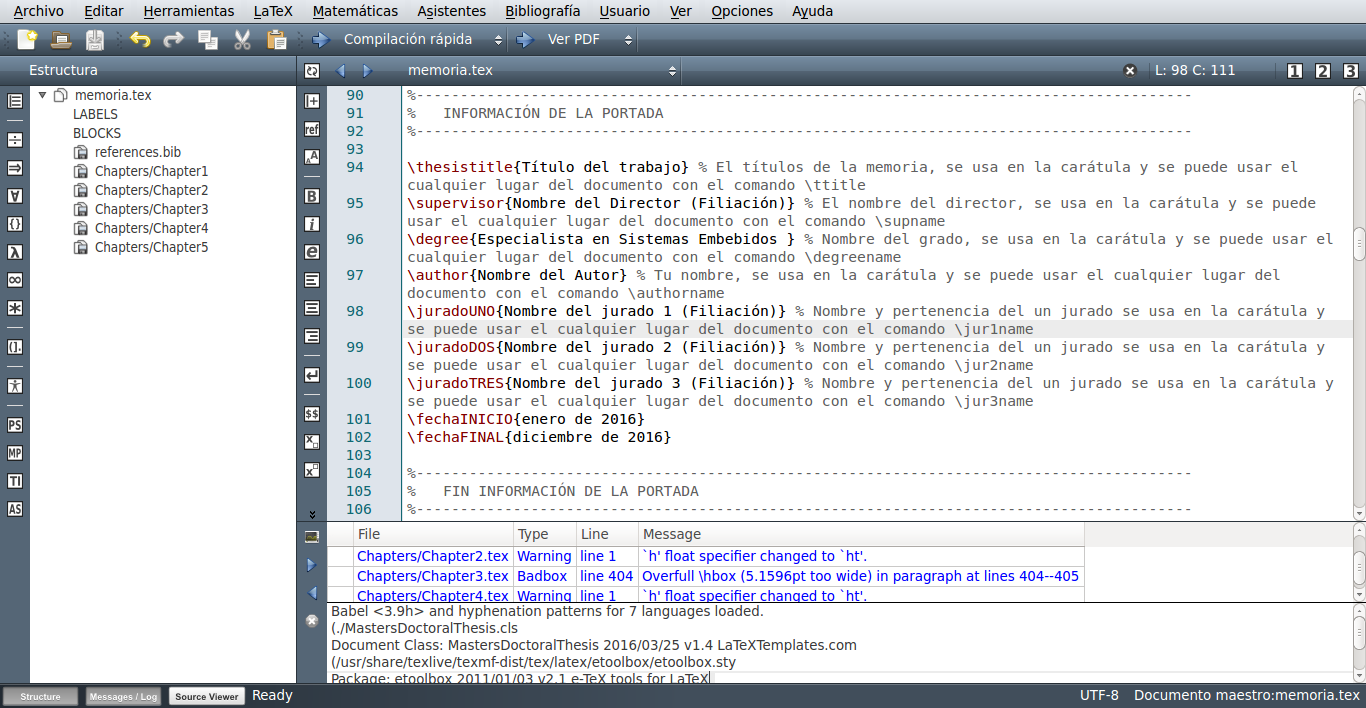
\includegraphics[width=\textwidth]{./Figures/texmaker.png}
	\caption{Entorno de trabajo de texMaker.}
	\label{fig:texmaker}
\end{figure}

Notar que existe una vista llamada Estructura a la izquierda de la interface que nos permite abrir desde dentro del programa los archivos individuales de los capítulos.  A la derecha se encuentra una vista con el archivo propiamente dicho para su edición. Hacia la parte inferior se encuentra una vista del log con información de los resultados de la compilación.  En esta última vista pueden aparecen advertencias o \textit{warning}, que normalmente pueden ser ignorados, y los errores que se indican en color rojo y deben resolverse para que se genere el PDF de salida.

Recordar que el archivo que se debe compilar con PDFLaTeX es \file{memoria.tex}, si se tratara de compilar alguno de los capítulos saldría un error.  Para salvar la molestia de tener que cambiar de archivo para compilar cada vez que se realice una modificación en un capítulo, se puede definir el archivo \file{memoria.tex} como ``documento maestro'' yendo al menú opciones -> ``definir documento actual como documento maestro'', lo que permite compilar con PDFLaTeX memoria.tex directamente desde cualquier archivo que se esté modificando . Se muestra esta opción en la figura \ref{fig:docMaestro}.

\begin{figure}[h]
	\centering
	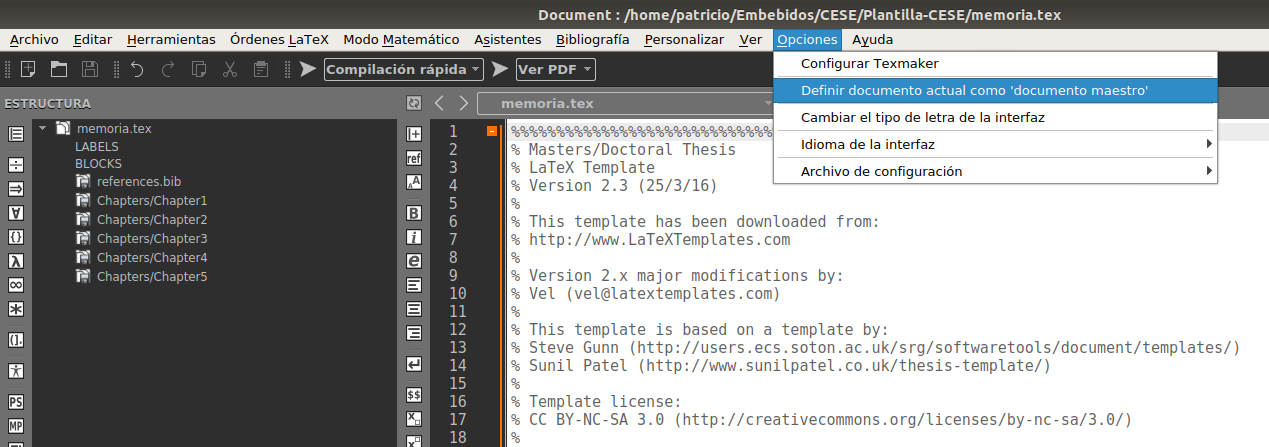
\includegraphics[width=\textwidth]{./Figures/docMaestro.png}
	\caption{Definir memoria.tex como documento maestro.}
	\label{fig:docMaestro}
\end{figure}

En el menú herramientas se encuentran las opciones de compilación.  Para producir un archivo PDF a partir de un archivo .tex se debe ejecutar PDFLaTeX (el shortcut es F6). Para incorporar nueva bibliografía se debe utilizar la opción BibTeX del mismo menú herramientas (el shortcut es F11).

Notar que para actualizar las tablas de contenidos se debe ejecutar PDFLaTeX dos veces.  Esto se debe a que es necesario actualizar algunos archivos auxiliares antes de obtener el resultado final.  En forma similar, para actualizar las referecias se debe ejecutar primero PDFLaTeX, después BibTeX y finalmente PDFLaTeX dos veces por idénticos motivos.

\section{Personalizando la plantilla, el archivo \file{memoria.tex}}
\label{sec:FillingFile}

Para personalizar la plantilla se debe incorporar la información propia en los distintos archivos \file{.tex}. 

Primero abrir \file{memoria.tex} con TexMaker (o el editor de su preferencia). Se debe ubicar dentro del archivo el bloque de código titulado \emph{INFORMACIÓN DE LA PORTADA} donde se deben incorporar los primeros datos personales con los que se constuirá automáticamente la portada.


%----------------------------------------------------------------------------------------

\section{El código del archivo \file{memoria.tex} explicado}

El archivo \file{memoria.tex} contiene la estructura del documento y es el archivo de mayor jeraquía de la memoria.  Podría ser equiparable a la función \emph{main()} de un programa en C, o mejor dicho al archivo fuente .c donde se encuentra definida la función main().

La estructura básica de cualquier documento de \LaTeX{} comienza con la definición de clase del documento, es seguida por un preámbulo donde se pueden agregar funcionalidades con el uso de \texttt{paquetes} (equiparables a bibliotecas de C), y finalmente, termina con el cuerpo del documento, donde irá el contenido de la memoria.

\lstset{%
  basicstyle=\small\ttfamily,
  language=[LaTeX]{TeX}
}

\begin{lstlisting}
\documentclass{article}  <- Definicion de clase
\usepackage{listings}	 <- Preambulo

\begin{document}	 <- Comienzo del contenido propio 
	Hello world!
\end{document}
\end{lstlisting}


El archivo \file{memoria.tex} se encuentra densamente comentado para explicar qué páginas, secciones y elementos de formato está creando el código \LaTeX{} en cada línea. El código está dividido en bloques con nombres en mayúsculas para que resulte evidente qué es lo que hace esa porción de código en particular. Inicialmente puede parecer que hay mucho código \LaTeX{}, pero es principalmente código para dar formato a la memoria por lo que no requiere intervención del usuario de la plantilla.  Sí se deben personalizar con su información los bloques indicados como:

\begin{itemize}
	\item Informacion de la memoria
	\item Carátula
	\item Resumen
	\item Agradecimientos
	\item Dedicatoria
\end{itemize}

El índice de contenidos, las listas de figura de tablas se generan en forma automática y no requieren intervención ni edición manual por parte del usuario de la plantilla. 

En la parte final del documento se encuentran los capítulos y los apéndices.  Por defecto se incluyen los 5 capítulos propuestos que se encuentran en la carpeta /Chapters. Cada capítulo se debe escribir en un archivo .tex separado y se debe poner en la carpeta \emph{Chapters} con el nombre \file{Chapter1}, \file{Chapter2}, etc\ldots El código para incluir capítulos desde archivos externos se muestra a continuación.

\begin{verbatim}
	% Chapter 1

\chapter{Introducción General} % Main chapter title

\label{Chapter1} % For referencing the chapter elsewhere, use \ref{Chapter1} 
\label{IntroGeneral}

%----------------------------------------------------------------------------------------

% Define some commands to keep the formatting separated from the content 
\newcommand{\keyword}[1]{\textbf{#1}}
\newcommand{\tabhead}[1]{\textbf{#1}}
\newcommand{\code}[1]{\texttt{#1}}
\newcommand{\file}[1]{\texttt{\bfseries#1}}
\newcommand{\option}[1]{\texttt{\itshape#1}}
\newcommand{\grados}{$^{\circ}$}

%----------------------------------------------------------------------------------------

%\section{Introducción}

%----------------------------------------------------------------------------------------
\section{Aprendiendo \LaTeX{}}

\LaTeX{} no es \textsc{WYSIWYG} (What You See is What You Get), a diferencia de los procesadores de texto como Microsoft Word o Pages de Apple o incluso LibreOffice en el mundo open-source. En lugar de ello, un documento escrito para \LaTeX{} es en realidad un archivo de texto simple, llano que \emph{no contiene formato} . Nosotros le decimos a \LaTeX{} cómo deseamos que se aplique el formato en el documento final escribiendo comandos simples entre el texto, por ejemplo, si quiero usar \emph{texto en cursiva para dar énfasis}, escribo \verb|\emph{texto}| y pongo el texto en cursiva que quiero entre medio de las llaves. Esto significa que \LaTeX{} es un lenguaje del tipo \enquote{mark-up}, muy parecido a HTML.

\subsection{Una introducción (no tan corta) a \LaTeX{}}

Si usted es nuevo a \LaTeX{}, hay un muy buen libro electrónico - disponible gratuitamente en Internet como un archivo PDF - llamado, \enquote{A (not so short) Introduction to \LaTeX{}}. El título del libro es generalmente acortado a simplemente \emph{lshort}. Puede descargar la versión más reciente en inglés (ya que se actualiza de vez en cuando) desde aquí:
\url{http://www.ctan.org/tex-archive/info/lshort/english/lshort.pdf}

Está disponible en varios idiomas además del inglés. Se puede encontrar la versión en español en la lista en esta página: \url{http://www.ctan.org/tex-archive/info/lshort/}


\subsection{Guía matemática rápida para \LaTeX{}}

Si usted está escribiendo un documento con mucho contenido matemático, entonces es posible que desee leer el documento de la AMS (American Mathematical Society) llamado, \enquote{A Short Math Guide for \LaTeX{}}. Se puede encontrar en línea en el siguiente link: \url{http://www.ams.org/tex/amslatex.html} en la sección \enquote{Additional Documentation} hacia la parte inferior de la página.


%----------------------------------------------------------------------------------------

\section{Utilizando esta plantilla}

Si usted está familiarizado con \LaTeX{}, entonces puede explorar la estructura de directorios de esta plantilla y proceder a personalizarla agregando su información en el bloque \emph{INFORMACIÓN DE LA PORTADA} en el archivo \file{memoria.tex}.  

Se puede continuar luego modificando el resto de los archivos siguiendo los lineamientos que se describen en la sección \ref{sec:FillingFile} en la página \pageref{sec:FillingFile}.

Asegúrese de leer el capítulo \ref{Chapter2} acerca de las convenciones utilizadas para las Memoria de los Trabajos Finales de la Carrera de Especialización en Sistemas Embebidos de FIUBA.

Si es nuevo en \LaTeX{} se recomienda que continue leyendo el documento ya que contiene información básica para aprovechar el potencial de esta herramienta.


\subsection{Acerca de esta plantilla}

Esta plantilla \LaTeX{} está basada originalmente en torno a un archivo de estilo \LaTeX{} creado por Steve R.\ Gunn de la  University of Southampton (UK), department of Electronics and Computer Science. Se puede encontrar su trabajo original en el siguiente sitio de internet:
\url{http://www.ecs.soton.ac.uk/~srg/softwaretools/document/templates/}

El archivo de Gunn, \file{ecsthesis.cls} fue posteriormente modificado por Sunil Patel quien creó una plantilla esqueleto con la estructura de carpetas. El template resultante se puede encontrar en el sitio web de Sunil Patel:
\url{http://www.sunilpatel.co.uk/thesis-template}

El template de Patel se publicó a través de  \url{http://www.LaTeXTemplates.com} desde donde fue modificado muchas veces en base a solicitudes de usuarios. La versión 2.0 y subsiguientes representan cambios significativos respecto a la versión de la plantilla modificada por Patel, que es de hecho, dificilmente reconocible. El trabajo en la version 2.0 fue realizado por Vel Gayevskiy y Johannes Böttcher.

Para la Carrera de Especialización en Sistemas Embebidos de FIUBA, la versión versión 2.3 fue modificada por el Ing. \href{mailto:pbos@fi.uba.ar}{Patricio Bos} para crear una plantilla fuertemente adaptada a la carrera de especialización.

%----------------------------------------------------------------------------------------

\section{Qué incluye esta plantilla}

\subsection{Carpetas}

Esta plantilla se distribuye como una único archivo .zip que se puede descomprimir en varios archivos y carpetas. Los nombres de las carpetas son (o pretender ser) auto-explicativos.

\keyword{Appendices} -- Esta es la carpeta donde se deben poner los apéndices. Cada apéndice debe ir en su propio archivo \file{.tex}. Se incluye un ejemplo y una plantilla en la carpeta.

\keyword{Chapters} -- Esta es la carpeta donde se deben poner los capítulos de la memoria. Cada capítulo debe ir un su propio archivo \file{.tex} por separado.  Se ofrece por defecto, la siguiente estructura de capítulos y se recomienda su utilización dentro de lo posible:

\begin{itemize}
\item Capítulo 1: Introducción general	
\item Capítulo 2: Introducción específica
\item Capítulo 3: Diseño e implementación
\item Capítulo 4: Ensayos y resultados
\item Capítulo 5: Conclusiones

\end{itemize}

Esta estructura de capítulos es la que se recomienda para las memorias de la especialización.

\keyword{Figures} -- Esta carpeta contiene todas las figuras de la memoria.  Estas son las versiones finales de las imágenes que van a ser incluidas en la memoria.  Pueden ser imágenes en formato \textit{raster}\footnote{\url{https://en.wikipedia.org/wiki/Raster_graphics}} como \file{.png}, \file{.jpg} o en formato vectoriales\footnote{\url{https://en.wikipedia.org/wiki/Vector_graphics}} como \file{.pdf}, \file{.ps}.  Se debe notar que utilizar imágenes vectoriales disminuye notablemente el peso del documento final y acelera el tiempo de compilación por lo que es recomendable su utilización siempre que sea posible.

\subsection{Archivos}

También están incluidos varios archivos, la mayoría de ellos son de texto plano y se puede ver su contenido en un editor de texto. Después de la compilación inicial, se verá que más archivos auxiliares son creados por \ LaTeX{} o BibTeX, pero son de uso interno y que no es necesario eliminarlos o hacer nada con ellos.  Toda la información necesaria para complilar el documento se encuentra en los archivos \file{.tex} y en las imágenes de la carpeta Figures.

\keyword{referencias.bib} - este es un archivo importante que contiene toda la información de referencias bibliográficas que se utilizarán para las citas en la memoria en conjunto con BibTeX. Usted puede escribir las entradas bibliográficas en forma manual, aunque existen también programas de gestión de referencias que facilitan la creación y gestión de las referencias y permiten exportarlas en formato BibTeX.  También hay disponibles sitios web como \url{books.google.com} que permiten obtener toda la información necesaria para una cita en formato BibTeX. Ver sección \ref{sec:biblio}

\keyword{MastersDoctoralThesis.cls} -- este es un archivo importante. Es el archivos con la clase que le informa a \LaTeX{} cómo debe dar formato a la memoria. El usuario de la plantilla no debería necesitar modificar nada de este archivo.

\keyword{memoria.pdf} -- esta es su memoria con una tipografía bellamente compuesta (en formato de archivo PDF) creado por \LaTeX{}. Se distribuye con la plantilla y después de compilar por primera vez sin hacer ningún cambio se debería obtener una versión idéntica a este documento.

\keyword{memoria.tex} -- este es un archivo importante. Este es el archivo que tiene que compilar \LaTeX{} para producir la memoria como un archivo PDF. Contiene un marco de trabajo y estructuras que le indican a \LaTeX{} cómo diagramar la memoria.  Está altamente comentado para que se pueda entender qué es lo que realiza cada línea de código y por qué está incluida en ese lugar.  En este archivo se debe completar la información personalizada de las primeras sección según se indica en la sección \ref{sec:FillingFile}.

Archivos que \emph{no} forman parte de la distribución de la plantilla pero que son generados por \LaTeX{} como archivos auxiliares necesarios para la producción de la memoria.pdf son:

\keyword{memoria.aux} -- este es un archivo auxiliar generado por \LaTeX{}, si se borra \LaTeX{} simplemente lo regenera cuando se compila el archivo principal \file{memoria.tex}.

\keyword{memoria.bbl} -- este es un archivo auxiliar generado por BibTeX, si se borra BibTeX simplemente lo regenera cuando se compila el archivo principal \file{memoria.tex}. Mientras que el archivo \file{.bib} contiene todas las referencias que hay, este archivo \file{.bbl} contine sólo las referencias que han sido citadas y se utiliza para la construcción de la bibiografía.

\keyword{memoria.blg} -- este es un archivo auxiliar generado por BibTeX, si se borra BibTeX simplemente lo regenera cuando se compila el archivo principal \file{memoria.tex}.

\keyword{memoria.lof} -- este es un archivo auxiliar generado por \LaTeX{}, si se borra \LaTeX{} simplemente lo regenera cuando se compila el archivo principal \file{memoria.tex}.  Le indica a \LaTeX{} cómo construir la sección \emph{Lista de Figuras}.
 
\keyword{memoria.log} --  este es un archivo auxiliar generado por \LaTeX{}, si se borra \LaTeX{} simplemente lo regenera cuando se compila el archivo principal \file{memoria.tex}. Contiene mensajes de \LaTeX{}. Si se reciben errores o advertencias durante la compilación, se guardan en este archivo \file{.log}.

\keyword{memoria.lot} -- este es un archivo auxiliar generado por \LaTeX{}, si se borra \LaTeX{} simplemente lo regenera cuando se compila el archivo principal \file{memoria.tex}.  Le indica a \LaTeX{} cómo construir la sección \emph{Lista de Tablas}.

\keyword{memoria.out} -- este es un archivo auxiliar generado por \LaTeX{}, si se borra \LaTeX{} simplemente lo regenera cuando se compila el archivo principal \file{memoria.tex}.

De esta larga lista de archivos, sólo aquellos con la extensión \file{.bib}, \file{.cls} y \file{.tex} son importantes.  Los otros archivos auxiliares pueden ser ignorados o borrados ya que \LaTeX{} y BibTeX los regenerarán durante la compilación.

%----------------------------------------------------------------------------------------

\section{Entorno de trabajo}

Ante de comenzar a editar la plantilla debemos tener un editor \LaTeX{} instalado en nuestra computadora.  En forma análoga a lo que sucede en lenguaje C, que se puede crear y editar código con casi cualquier editor, exiten ciertos entornos de trabajo que nos pueden simplificar mucho la tarea.  En este sentido, se recomienda, sobre todo para los principiantes en \LaTeX{} la utilización de TexMaker, un programa gratuito y multi-plantaforma que está disponible tanto para windows como para sistemas GNU/linux.

La versión más reciente de TexMaker es la 4.5 y se puede descargar del siguiente link: \url{http://www.xm1math.net/texmaker/download.html}. Se puede consultar el manual de usuario en el siguiente link: \url{http://www.xm1math.net/texmaker/doc.html}.
 

\subsection{Paquetes adicionales}

Si bien durante el proceso de instalación de TexMaker, o cualquier otro editor que se haya elegido, se instalarán en el sistema los paquetes básicos necesarios para trabajar con \LaTeX{}, la plantilla de los trabajos de Especialización y Maestría requieren de paquete adicionales.

Se indican a continuación los comandos que se deben introducir en la consola de Ubuntu (ctrl + alt + t) para instalarlos:

\begin{lstlisting}[language=bash]
  $ sudo apt install texlive-lang-spanish texlive-science 
  $ sudo apt install texlive-bibtex-extra biber
  $ sudo apt install texlive texlive-fonts-recommended
  $ sudo apt install texlive-latex-extra
\end{lstlisting}


\subsection{Configurando TexMaker}


Una vez instalado el programa y los paquetes adicionales se debe abrir el archivo memoria.tex con el editor para ver una pantalla similar a la que se puede apreciar en la figura \ref{fig:texmaker}. 

\begin{figure}[h]
	\centering
	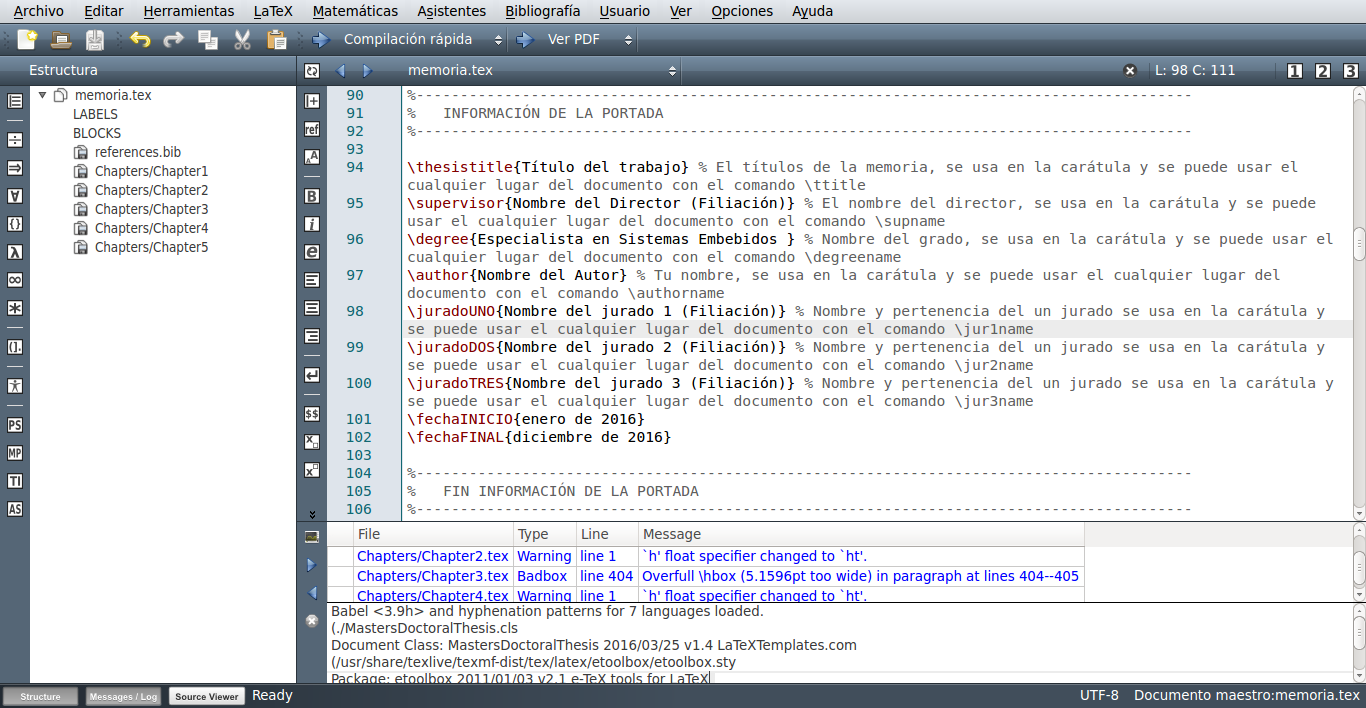
\includegraphics[width=\textwidth]{./Figures/texmaker.png}
	\caption{Entorno de trabajo de texMaker.}
	\label{fig:texmaker}
\end{figure}

Notar que existe una vista llamada Estructura a la izquierda de la interface que nos permite abrir desde dentro del programa los archivos individuales de los capítulos.  A la derecha se encuentra una vista con el archivo propiamente dicho para su edición. Hacia la parte inferior se encuentra una vista del log con información de los resultados de la compilación.  En esta última vista pueden aparecen advertencias o \textit{warning}, que normalmente pueden ser ignorados, y los errores que se indican en color rojo y deben resolverse para que se genere el PDF de salida.

Recordar que el archivo que se debe compilar con PDFLaTeX es \file{memoria.tex}, si se tratara de compilar alguno de los capítulos saldría un error.  Para salvar la molestia de tener que cambiar de archivo para compilar cada vez que se realice una modificación en un capítulo, se puede definir el archivo \file{memoria.tex} como ``documento maestro'' yendo al menú opciones -> ``definir documento actual como documento maestro'', lo que permite compilar con PDFLaTeX memoria.tex directamente desde cualquier archivo que se esté modificando . Se muestra esta opción en la figura \ref{fig:docMaestro}.

\begin{figure}[h]
	\centering
	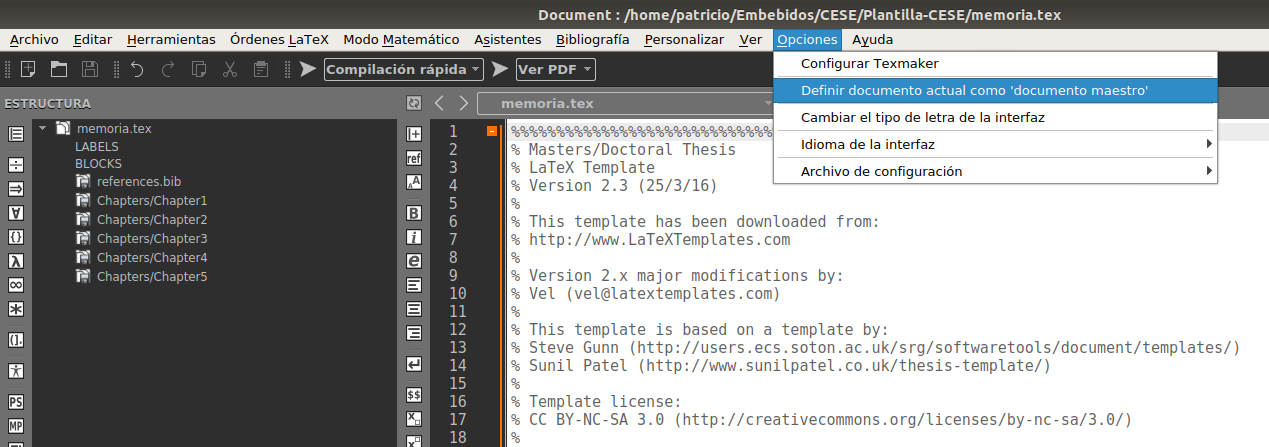
\includegraphics[width=\textwidth]{./Figures/docMaestro.png}
	\caption{Definir memoria.tex como documento maestro.}
	\label{fig:docMaestro}
\end{figure}

En el menú herramientas se encuentran las opciones de compilación.  Para producir un archivo PDF a partir de un archivo .tex se debe ejecutar PDFLaTeX (el shortcut es F6). Para incorporar nueva bibliografía se debe utilizar la opción BibTeX del mismo menú herramientas (el shortcut es F11).

Notar que para actualizar las tablas de contenidos se debe ejecutar PDFLaTeX dos veces.  Esto se debe a que es necesario actualizar algunos archivos auxiliares antes de obtener el resultado final.  En forma similar, para actualizar las referecias se debe ejecutar primero PDFLaTeX, después BibTeX y finalmente PDFLaTeX dos veces por idénticos motivos.

\section{Personalizando la plantilla, el archivo \file{memoria.tex}}
\label{sec:FillingFile}

Para personalizar la plantilla se debe incorporar la información propia en los distintos archivos \file{.tex}. 

Primero abrir \file{memoria.tex} con TexMaker (o el editor de su preferencia). Se debe ubicar dentro del archivo el bloque de código titulado \emph{INFORMACIÓN DE LA PORTADA} donde se deben incorporar los primeros datos personales con los que se constuirá automáticamente la portada.


%----------------------------------------------------------------------------------------

\section{El código del archivo \file{memoria.tex} explicado}

El archivo \file{memoria.tex} contiene la estructura del documento y es el archivo de mayor jeraquía de la memoria.  Podría ser equiparable a la función \emph{main()} de un programa en C, o mejor dicho al archivo fuente .c donde se encuentra definida la función main().

La estructura básica de cualquier documento de \LaTeX{} comienza con la definición de clase del documento, es seguida por un preámbulo donde se pueden agregar funcionalidades con el uso de \texttt{paquetes} (equiparables a bibliotecas de C), y finalmente, termina con el cuerpo del documento, donde irá el contenido de la memoria.

\lstset{%
  basicstyle=\small\ttfamily,
  language=[LaTeX]{TeX}
}

\begin{lstlisting}
\documentclass{article}  <- Definicion de clase
\usepackage{listings}	 <- Preambulo

\begin{document}	 <- Comienzo del contenido propio 
	Hello world!
\end{document}
\end{lstlisting}


El archivo \file{memoria.tex} se encuentra densamente comentado para explicar qué páginas, secciones y elementos de formato está creando el código \LaTeX{} en cada línea. El código está dividido en bloques con nombres en mayúsculas para que resulte evidente qué es lo que hace esa porción de código en particular. Inicialmente puede parecer que hay mucho código \LaTeX{}, pero es principalmente código para dar formato a la memoria por lo que no requiere intervención del usuario de la plantilla.  Sí se deben personalizar con su información los bloques indicados como:

\begin{itemize}
	\item Informacion de la memoria
	\item Carátula
	\item Resumen
	\item Agradecimientos
	\item Dedicatoria
\end{itemize}

El índice de contenidos, las listas de figura de tablas se generan en forma automática y no requieren intervención ni edición manual por parte del usuario de la plantilla. 

En la parte final del documento se encuentran los capítulos y los apéndices.  Por defecto se incluyen los 5 capítulos propuestos que se encuentran en la carpeta /Chapters. Cada capítulo se debe escribir en un archivo .tex separado y se debe poner en la carpeta \emph{Chapters} con el nombre \file{Chapter1}, \file{Chapter2}, etc\ldots El código para incluir capítulos desde archivos externos se muestra a continuación.

\begin{verbatim}
	% Chapter 1

\chapter{Introducción General} % Main chapter title

\label{Chapter1} % For referencing the chapter elsewhere, use \ref{Chapter1} 
\label{IntroGeneral}

%----------------------------------------------------------------------------------------

% Define some commands to keep the formatting separated from the content 
\newcommand{\keyword}[1]{\textbf{#1}}
\newcommand{\tabhead}[1]{\textbf{#1}}
\newcommand{\code}[1]{\texttt{#1}}
\newcommand{\file}[1]{\texttt{\bfseries#1}}
\newcommand{\option}[1]{\texttt{\itshape#1}}
\newcommand{\grados}{$^{\circ}$}

%----------------------------------------------------------------------------------------

%\section{Introducción}

%----------------------------------------------------------------------------------------
\section{Aprendiendo \LaTeX{}}

\LaTeX{} no es \textsc{WYSIWYG} (What You See is What You Get), a diferencia de los procesadores de texto como Microsoft Word o Pages de Apple o incluso LibreOffice en el mundo open-source. En lugar de ello, un documento escrito para \LaTeX{} es en realidad un archivo de texto simple, llano que \emph{no contiene formato} . Nosotros le decimos a \LaTeX{} cómo deseamos que se aplique el formato en el documento final escribiendo comandos simples entre el texto, por ejemplo, si quiero usar \emph{texto en cursiva para dar énfasis}, escribo \verb|\emph{texto}| y pongo el texto en cursiva que quiero entre medio de las llaves. Esto significa que \LaTeX{} es un lenguaje del tipo \enquote{mark-up}, muy parecido a HTML.

\subsection{Una introducción (no tan corta) a \LaTeX{}}

Si usted es nuevo a \LaTeX{}, hay un muy buen libro electrónico - disponible gratuitamente en Internet como un archivo PDF - llamado, \enquote{A (not so short) Introduction to \LaTeX{}}. El título del libro es generalmente acortado a simplemente \emph{lshort}. Puede descargar la versión más reciente en inglés (ya que se actualiza de vez en cuando) desde aquí:
\url{http://www.ctan.org/tex-archive/info/lshort/english/lshort.pdf}

Está disponible en varios idiomas además del inglés. Se puede encontrar la versión en español en la lista en esta página: \url{http://www.ctan.org/tex-archive/info/lshort/}


\subsection{Guía matemática rápida para \LaTeX{}}

Si usted está escribiendo un documento con mucho contenido matemático, entonces es posible que desee leer el documento de la AMS (American Mathematical Society) llamado, \enquote{A Short Math Guide for \LaTeX{}}. Se puede encontrar en línea en el siguiente link: \url{http://www.ams.org/tex/amslatex.html} en la sección \enquote{Additional Documentation} hacia la parte inferior de la página.


%----------------------------------------------------------------------------------------

\section{Utilizando esta plantilla}

Si usted está familiarizado con \LaTeX{}, entonces puede explorar la estructura de directorios de esta plantilla y proceder a personalizarla agregando su información en el bloque \emph{INFORMACIÓN DE LA PORTADA} en el archivo \file{memoria.tex}.  

Se puede continuar luego modificando el resto de los archivos siguiendo los lineamientos que se describen en la sección \ref{sec:FillingFile} en la página \pageref{sec:FillingFile}.

Asegúrese de leer el capítulo \ref{Chapter2} acerca de las convenciones utilizadas para las Memoria de los Trabajos Finales de la Carrera de Especialización en Sistemas Embebidos de FIUBA.

Si es nuevo en \LaTeX{} se recomienda que continue leyendo el documento ya que contiene información básica para aprovechar el potencial de esta herramienta.


\subsection{Acerca de esta plantilla}

Esta plantilla \LaTeX{} está basada originalmente en torno a un archivo de estilo \LaTeX{} creado por Steve R.\ Gunn de la  University of Southampton (UK), department of Electronics and Computer Science. Se puede encontrar su trabajo original en el siguiente sitio de internet:
\url{http://www.ecs.soton.ac.uk/~srg/softwaretools/document/templates/}

El archivo de Gunn, \file{ecsthesis.cls} fue posteriormente modificado por Sunil Patel quien creó una plantilla esqueleto con la estructura de carpetas. El template resultante se puede encontrar en el sitio web de Sunil Patel:
\url{http://www.sunilpatel.co.uk/thesis-template}

El template de Patel se publicó a través de  \url{http://www.LaTeXTemplates.com} desde donde fue modificado muchas veces en base a solicitudes de usuarios. La versión 2.0 y subsiguientes representan cambios significativos respecto a la versión de la plantilla modificada por Patel, que es de hecho, dificilmente reconocible. El trabajo en la version 2.0 fue realizado por Vel Gayevskiy y Johannes Böttcher.

Para la Carrera de Especialización en Sistemas Embebidos de FIUBA, la versión versión 2.3 fue modificada por el Ing. \href{mailto:pbos@fi.uba.ar}{Patricio Bos} para crear una plantilla fuertemente adaptada a la carrera de especialización.

%----------------------------------------------------------------------------------------

\section{Qué incluye esta plantilla}

\subsection{Carpetas}

Esta plantilla se distribuye como una único archivo .zip que se puede descomprimir en varios archivos y carpetas. Los nombres de las carpetas son (o pretender ser) auto-explicativos.

\keyword{Appendices} -- Esta es la carpeta donde se deben poner los apéndices. Cada apéndice debe ir en su propio archivo \file{.tex}. Se incluye un ejemplo y una plantilla en la carpeta.

\keyword{Chapters} -- Esta es la carpeta donde se deben poner los capítulos de la memoria. Cada capítulo debe ir un su propio archivo \file{.tex} por separado.  Se ofrece por defecto, la siguiente estructura de capítulos y se recomienda su utilización dentro de lo posible:

\begin{itemize}
\item Capítulo 1: Introducción general	
\item Capítulo 2: Introducción específica
\item Capítulo 3: Diseño e implementación
\item Capítulo 4: Ensayos y resultados
\item Capítulo 5: Conclusiones

\end{itemize}

Esta estructura de capítulos es la que se recomienda para las memorias de la especialización.

\keyword{Figures} -- Esta carpeta contiene todas las figuras de la memoria.  Estas son las versiones finales de las imágenes que van a ser incluidas en la memoria.  Pueden ser imágenes en formato \textit{raster}\footnote{\url{https://en.wikipedia.org/wiki/Raster_graphics}} como \file{.png}, \file{.jpg} o en formato vectoriales\footnote{\url{https://en.wikipedia.org/wiki/Vector_graphics}} como \file{.pdf}, \file{.ps}.  Se debe notar que utilizar imágenes vectoriales disminuye notablemente el peso del documento final y acelera el tiempo de compilación por lo que es recomendable su utilización siempre que sea posible.

\subsection{Archivos}

También están incluidos varios archivos, la mayoría de ellos son de texto plano y se puede ver su contenido en un editor de texto. Después de la compilación inicial, se verá que más archivos auxiliares son creados por \ LaTeX{} o BibTeX, pero son de uso interno y que no es necesario eliminarlos o hacer nada con ellos.  Toda la información necesaria para complilar el documento se encuentra en los archivos \file{.tex} y en las imágenes de la carpeta Figures.

\keyword{referencias.bib} - este es un archivo importante que contiene toda la información de referencias bibliográficas que se utilizarán para las citas en la memoria en conjunto con BibTeX. Usted puede escribir las entradas bibliográficas en forma manual, aunque existen también programas de gestión de referencias que facilitan la creación y gestión de las referencias y permiten exportarlas en formato BibTeX.  También hay disponibles sitios web como \url{books.google.com} que permiten obtener toda la información necesaria para una cita en formato BibTeX. Ver sección \ref{sec:biblio}

\keyword{MastersDoctoralThesis.cls} -- este es un archivo importante. Es el archivos con la clase que le informa a \LaTeX{} cómo debe dar formato a la memoria. El usuario de la plantilla no debería necesitar modificar nada de este archivo.

\keyword{memoria.pdf} -- esta es su memoria con una tipografía bellamente compuesta (en formato de archivo PDF) creado por \LaTeX{}. Se distribuye con la plantilla y después de compilar por primera vez sin hacer ningún cambio se debería obtener una versión idéntica a este documento.

\keyword{memoria.tex} -- este es un archivo importante. Este es el archivo que tiene que compilar \LaTeX{} para producir la memoria como un archivo PDF. Contiene un marco de trabajo y estructuras que le indican a \LaTeX{} cómo diagramar la memoria.  Está altamente comentado para que se pueda entender qué es lo que realiza cada línea de código y por qué está incluida en ese lugar.  En este archivo se debe completar la información personalizada de las primeras sección según se indica en la sección \ref{sec:FillingFile}.

Archivos que \emph{no} forman parte de la distribución de la plantilla pero que son generados por \LaTeX{} como archivos auxiliares necesarios para la producción de la memoria.pdf son:

\keyword{memoria.aux} -- este es un archivo auxiliar generado por \LaTeX{}, si se borra \LaTeX{} simplemente lo regenera cuando se compila el archivo principal \file{memoria.tex}.

\keyword{memoria.bbl} -- este es un archivo auxiliar generado por BibTeX, si se borra BibTeX simplemente lo regenera cuando se compila el archivo principal \file{memoria.tex}. Mientras que el archivo \file{.bib} contiene todas las referencias que hay, este archivo \file{.bbl} contine sólo las referencias que han sido citadas y se utiliza para la construcción de la bibiografía.

\keyword{memoria.blg} -- este es un archivo auxiliar generado por BibTeX, si se borra BibTeX simplemente lo regenera cuando se compila el archivo principal \file{memoria.tex}.

\keyword{memoria.lof} -- este es un archivo auxiliar generado por \LaTeX{}, si se borra \LaTeX{} simplemente lo regenera cuando se compila el archivo principal \file{memoria.tex}.  Le indica a \LaTeX{} cómo construir la sección \emph{Lista de Figuras}.
 
\keyword{memoria.log} --  este es un archivo auxiliar generado por \LaTeX{}, si se borra \LaTeX{} simplemente lo regenera cuando se compila el archivo principal \file{memoria.tex}. Contiene mensajes de \LaTeX{}. Si se reciben errores o advertencias durante la compilación, se guardan en este archivo \file{.log}.

\keyword{memoria.lot} -- este es un archivo auxiliar generado por \LaTeX{}, si se borra \LaTeX{} simplemente lo regenera cuando se compila el archivo principal \file{memoria.tex}.  Le indica a \LaTeX{} cómo construir la sección \emph{Lista de Tablas}.

\keyword{memoria.out} -- este es un archivo auxiliar generado por \LaTeX{}, si se borra \LaTeX{} simplemente lo regenera cuando se compila el archivo principal \file{memoria.tex}.

De esta larga lista de archivos, sólo aquellos con la extensión \file{.bib}, \file{.cls} y \file{.tex} son importantes.  Los otros archivos auxiliares pueden ser ignorados o borrados ya que \LaTeX{} y BibTeX los regenerarán durante la compilación.

%----------------------------------------------------------------------------------------

\section{Entorno de trabajo}

Ante de comenzar a editar la plantilla debemos tener un editor \LaTeX{} instalado en nuestra computadora.  En forma análoga a lo que sucede en lenguaje C, que se puede crear y editar código con casi cualquier editor, exiten ciertos entornos de trabajo que nos pueden simplificar mucho la tarea.  En este sentido, se recomienda, sobre todo para los principiantes en \LaTeX{} la utilización de TexMaker, un programa gratuito y multi-plantaforma que está disponible tanto para windows como para sistemas GNU/linux.

La versión más reciente de TexMaker es la 4.5 y se puede descargar del siguiente link: \url{http://www.xm1math.net/texmaker/download.html}. Se puede consultar el manual de usuario en el siguiente link: \url{http://www.xm1math.net/texmaker/doc.html}.
 

\subsection{Paquetes adicionales}

Si bien durante el proceso de instalación de TexMaker, o cualquier otro editor que se haya elegido, se instalarán en el sistema los paquetes básicos necesarios para trabajar con \LaTeX{}, la plantilla de los trabajos de Especialización y Maestría requieren de paquete adicionales.

Se indican a continuación los comandos que se deben introducir en la consola de Ubuntu (ctrl + alt + t) para instalarlos:

\begin{lstlisting}[language=bash]
  $ sudo apt install texlive-lang-spanish texlive-science 
  $ sudo apt install texlive-bibtex-extra biber
  $ sudo apt install texlive texlive-fonts-recommended
  $ sudo apt install texlive-latex-extra
\end{lstlisting}


\subsection{Configurando TexMaker}


Una vez instalado el programa y los paquetes adicionales se debe abrir el archivo memoria.tex con el editor para ver una pantalla similar a la que se puede apreciar en la figura \ref{fig:texmaker}. 

\begin{figure}[h]
	\centering
	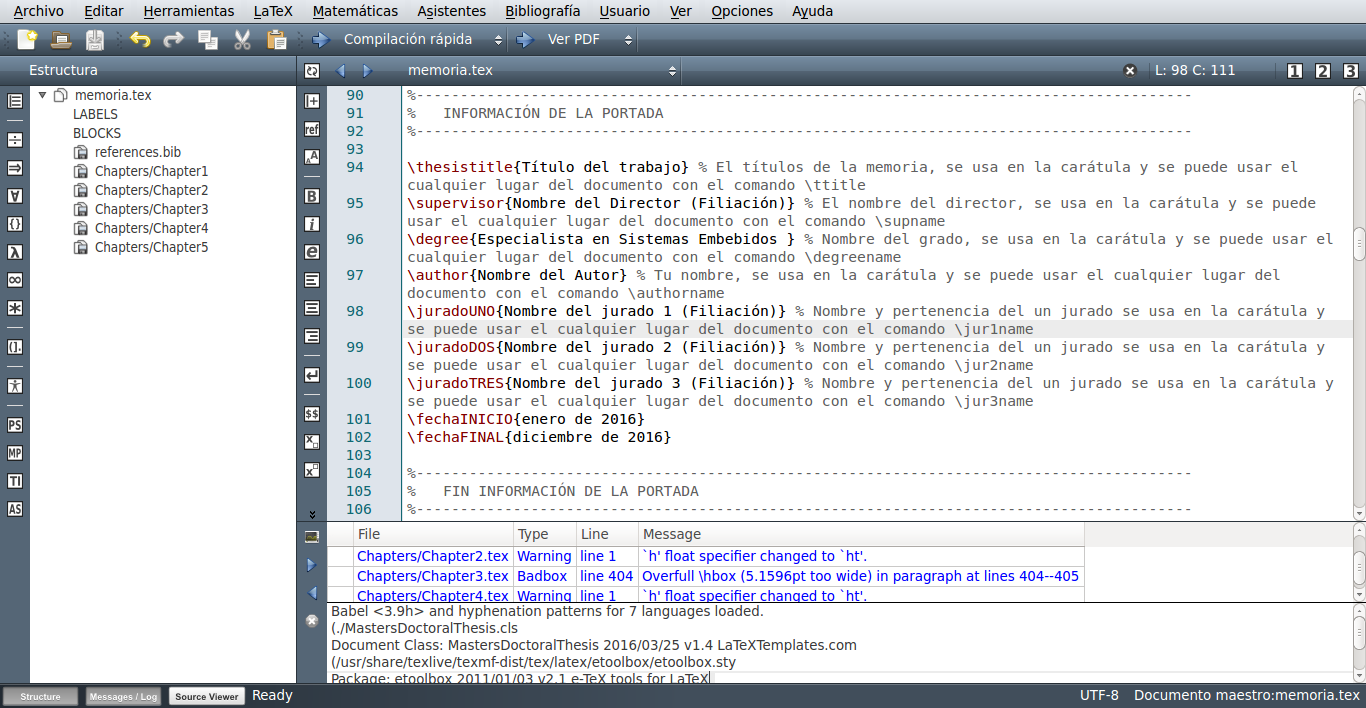
\includegraphics[width=\textwidth]{./Figures/texmaker.png}
	\caption{Entorno de trabajo de texMaker.}
	\label{fig:texmaker}
\end{figure}

Notar que existe una vista llamada Estructura a la izquierda de la interface que nos permite abrir desde dentro del programa los archivos individuales de los capítulos.  A la derecha se encuentra una vista con el archivo propiamente dicho para su edición. Hacia la parte inferior se encuentra una vista del log con información de los resultados de la compilación.  En esta última vista pueden aparecen advertencias o \textit{warning}, que normalmente pueden ser ignorados, y los errores que se indican en color rojo y deben resolverse para que se genere el PDF de salida.

Recordar que el archivo que se debe compilar con PDFLaTeX es \file{memoria.tex}, si se tratara de compilar alguno de los capítulos saldría un error.  Para salvar la molestia de tener que cambiar de archivo para compilar cada vez que se realice una modificación en un capítulo, se puede definir el archivo \file{memoria.tex} como ``documento maestro'' yendo al menú opciones -> ``definir documento actual como documento maestro'', lo que permite compilar con PDFLaTeX memoria.tex directamente desde cualquier archivo que se esté modificando . Se muestra esta opción en la figura \ref{fig:docMaestro}.

\begin{figure}[h]
	\centering
	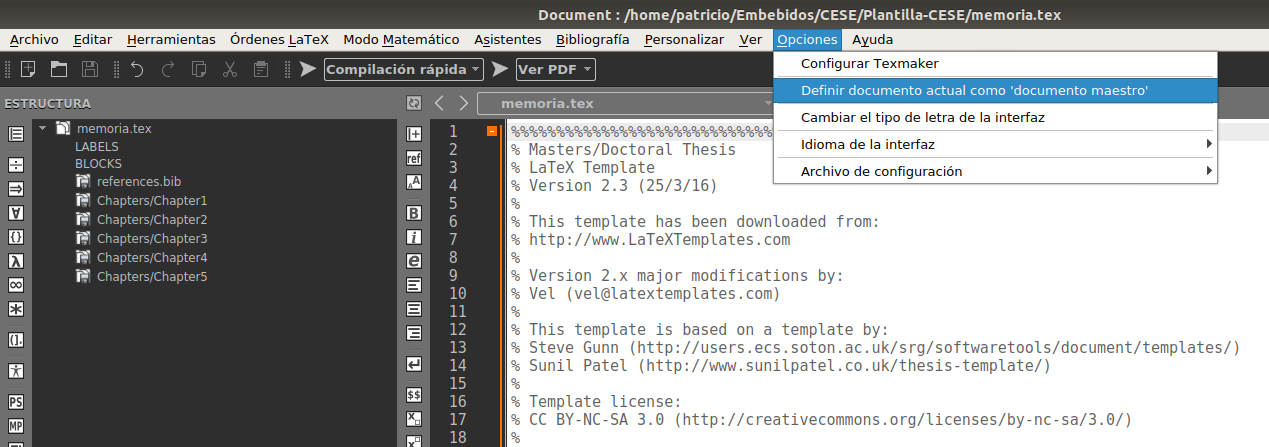
\includegraphics[width=\textwidth]{./Figures/docMaestro.png}
	\caption{Definir memoria.tex como documento maestro.}
	\label{fig:docMaestro}
\end{figure}

En el menú herramientas se encuentran las opciones de compilación.  Para producir un archivo PDF a partir de un archivo .tex se debe ejecutar PDFLaTeX (el shortcut es F6). Para incorporar nueva bibliografía se debe utilizar la opción BibTeX del mismo menú herramientas (el shortcut es F11).

Notar que para actualizar las tablas de contenidos se debe ejecutar PDFLaTeX dos veces.  Esto se debe a que es necesario actualizar algunos archivos auxiliares antes de obtener el resultado final.  En forma similar, para actualizar las referecias se debe ejecutar primero PDFLaTeX, después BibTeX y finalmente PDFLaTeX dos veces por idénticos motivos.

\section{Personalizando la plantilla, el archivo \file{memoria.tex}}
\label{sec:FillingFile}

Para personalizar la plantilla se debe incorporar la información propia en los distintos archivos \file{.tex}. 

Primero abrir \file{memoria.tex} con TexMaker (o el editor de su preferencia). Se debe ubicar dentro del archivo el bloque de código titulado \emph{INFORMACIÓN DE LA PORTADA} donde se deben incorporar los primeros datos personales con los que se constuirá automáticamente la portada.


%----------------------------------------------------------------------------------------

\section{El código del archivo \file{memoria.tex} explicado}

El archivo \file{memoria.tex} contiene la estructura del documento y es el archivo de mayor jeraquía de la memoria.  Podría ser equiparable a la función \emph{main()} de un programa en C, o mejor dicho al archivo fuente .c donde se encuentra definida la función main().

La estructura básica de cualquier documento de \LaTeX{} comienza con la definición de clase del documento, es seguida por un preámbulo donde se pueden agregar funcionalidades con el uso de \texttt{paquetes} (equiparables a bibliotecas de C), y finalmente, termina con el cuerpo del documento, donde irá el contenido de la memoria.

\lstset{%
  basicstyle=\small\ttfamily,
  language=[LaTeX]{TeX}
}

\begin{lstlisting}
\documentclass{article}  <- Definicion de clase
\usepackage{listings}	 <- Preambulo

\begin{document}	 <- Comienzo del contenido propio 
	Hello world!
\end{document}
\end{lstlisting}


El archivo \file{memoria.tex} se encuentra densamente comentado para explicar qué páginas, secciones y elementos de formato está creando el código \LaTeX{} en cada línea. El código está dividido en bloques con nombres en mayúsculas para que resulte evidente qué es lo que hace esa porción de código en particular. Inicialmente puede parecer que hay mucho código \LaTeX{}, pero es principalmente código para dar formato a la memoria por lo que no requiere intervención del usuario de la plantilla.  Sí se deben personalizar con su información los bloques indicados como:

\begin{itemize}
	\item Informacion de la memoria
	\item Carátula
	\item Resumen
	\item Agradecimientos
	\item Dedicatoria
\end{itemize}

El índice de contenidos, las listas de figura de tablas se generan en forma automática y no requieren intervención ni edición manual por parte del usuario de la plantilla. 

En la parte final del documento se encuentran los capítulos y los apéndices.  Por defecto se incluyen los 5 capítulos propuestos que se encuentran en la carpeta /Chapters. Cada capítulo se debe escribir en un archivo .tex separado y se debe poner en la carpeta \emph{Chapters} con el nombre \file{Chapter1}, \file{Chapter2}, etc\ldots El código para incluir capítulos desde archivos externos se muestra a continuación.

\begin{verbatim}
	\include{Chapters/Chapter1}
	\include{Chapters/Chapter2} 
	\include{Chapters/Chapter3}
	\include{Chapters/Chapter4} 
	\include{Chapters/Chapter5} 
\end{verbatim}

Los apéndices también deben escribirse en archivos .tex separados, que se deben ubicar dentro de la carpeta \emph{Appendices}. Los apéndices vienen comentados por defecto con el caracter \code{\%} y para incluirlos simplemente se debe eliminar dicho caracter.

Finalmente, se encuentra el código para incluir la bibliografía en el documento final.  Este código tampoco debe modificarse. La metodología para trabajar las referencias bibliográficas se desarrolla en la sección \ref{sec:biblio}.
%----------------------------------------------------------------------------------------

\section{Bibliografía}
\label{sec:biblio}

Las opciones de formato de la bibliografía se controlan a través del paquete de latex \option{biblatex} que se incluye en la memoria en el archivo memoria.tex.  Estas opciones determinan cómo se generan las citas bibliográficas en el cuerpo del documento y cómo se genera la biblografía al final de la memoria.

En el preámbulo se puede encontrar el código que incluye el paquete biblatex, que no requiere ninguna modificación del usuario de la plantilla, y que contiene las siguientes opciones:

\begin{lstlisting}
\usepackage[backend=bibtex,
	natbib=true, 
	style=numeric, 
	sorting=none]
{biblatex}
\end{lstlisting}

En el archivo \file{reference.bib} se encuentran las referencias bibliográficas que se pueden citar en el documento.  Para incorporar una nueva cita al documento lo primero es agregarla en este archivo con todos los campos necesario.  Todas las entradas bibliográficas comienzan con $@$ y una palabra que define el formato de la entrada.  Para cada formato existen campos obligatorios que deben completarse. No importa el orden en que las entradas estén definidas en el archivo .bib.  Tampoco es importante el orden en que estén definidos los campos de una entrada bibliográfica. A continuación se muestran algunos ejemplos:

\begin{lstlisting}
@ARTICLE{ARTICLE:1,
    AUTHOR="John Doe",
    TITLE="Title",
    JOURNAL="Journal",
    YEAR="2017",
}
\end{lstlisting}


\begin{lstlisting}
@BOOK{BOOK:1,
    AUTHOR="John Doe",
    TITLE="The Book without Title",
    PUBLISHER="Dummy Publisher",
    YEAR="2100",
}
\end{lstlisting}


\begin{lstlisting}
@INBOOK{BOOK:2,
    AUTHOR="John Doe",
    TITLE="The Book without Title",
    PUBLISHER="Dummy Publisher",
    YEAR="2100",
    PAGES="100-200",
}
\end{lstlisting}


\begin{lstlisting}
@MISC{WEBSITE:1,
    HOWPUBLISHED = "\url{http://example.com}",
    AUTHOR = "Intel",
    TITLE = "Example Website",
    MONTH = "12",
    YEAR = "1988",
    URLDATE = {2012-11-26}
}
\end{lstlisting}

Se debe notar que los nombres \emph{ARTICLE:1}, \emph{BOOK:1}, \emph{BOOK:2} y \emph{WEBSITE:1} son nombres de fantasía que le sirve al autor del documento para indentificar la entrada. En este sentido, se podrían reemplazar por cualquier otro nombre.  Tampoco es necesario poner : seguido de un número, en los ejemplos sólo se incluye como un posible estilo para identificar las entradas.

La entradas se citan en el documento con el comando: 

\begin{verbatim}
\citep{nombre_de_la_entrada}
\end{verbatim}

Y cuando se usan, se muestran así: \citep{ARTICLE:1}, \citep{BOOK:1}, \citep{BOOK:2}, \citep{WEBSITE:1}.  Notar cómo se conforma la sección Bibliografía al final del documento. 

	\chapter{Introducción Específica} % Main chapter title

\label{Chapter2}

%----------------------------------------------------------------------------------------
%	SECTION 1
%----------------------------------------------------------------------------------------

\section{Título de la sección con este uso de las mayúsculas}
\label{sec:ejemplo}
La idea de esta sección es presentar el tema de modo que cualquier persona que no conoce el tema pueda entender de qué se trata y por qué es importante realizar este trabajo y cuál es su impacto.

Si en el texto se hace alusión a diferentes partes del trabajo referirse a ellas como Capítulo, Sección o subsección según corresponda. Por ejemplo: ``En el Capítulo \ref{Chapter1} se explica tal cosa'', o ``En la Sección \ref{sec:ejemplo} se presenta lo que sea'', o ``En la la subsección \ref{subsec:ejemplo} se discute otra cosa''.

Entre párrafos sucesivos dejar un espacio, como el que se observa entre este párrafo y el anterior. Pero las oraciones de un mismo párrafo van en forma consecutiva, como se observa acá. Luego, cuando se quiere poner una lista tabulada se hace así:

\begin{itemize}
	\item Este es el primer elemento de la lista.
	\item Este es el segundo elemento de la lista.
\end{itemize}

Notar el uso de las mayúsculas y el punto al final de cada elemento.
Si se desea poner una lista numerada el formato es este:
\begin{enumerate}
	\item Este es el primer elemento de la lista.
	\item Este es el segundo elemento de la lista.
\end{enumerate}

Notar el uso de las mayúsculas y el punto al final de cada elemento.

\subsection{Este es el título de una subsección}
\label{subsec:ejemplo}

Se recomienda no utilizar \textbf{texto en negritas} en ningún párrafo, ni tampoco \underline{texto subrayado}. En cambio sí se sugiere utilizar \textit{texto en cursiva} donde se considere apropiado.

Se sugiere que la escritura sea impersonal. Por ejemplo, no utilizar ``el diseño del firmware lo hice de acuerdo con tal principio'', sino ``el firmware fue diseñado utilizando tal principio''. En lo posible hablar en tiempo pasado, ya que la memoria describe un trabajo que ya fue realizado.

Se recomienda no utilizar una sección de glosario sino colocar la descripción de las abreviaturas como parte del mismo cuerpo del texto. Por ejemplo, RTOS (\textit{Real Time Operating System}, Sistema Operativo de Tiempo Real) o en caso de considerarlo apropiado mediante notas a pie de página.

Si se desea indicar alguna página web utilizar el siguiente formato de referencias bibliográficas, dónde las referencias se detallan en la sección de bibliografía de la memoria,utilizado el formato establecido por IEEE en [1]. Por ejemplo, ``el presente trabajo se basa en la plataforma EDU-CIAA-NXP, la cual se describe en detalle en [2]''. 
 
	\chapter{Diseño e implementación} % Main chapter title

En este capítulo se van a describir las soluciones planteadas al problema resuelto en este trabajo.

%----------------------------------------------------------------------------------------
%	SECTION 1
%----------------------------------------------------------------------------------------
\section{Arquitectura del sistema}

En la figura \ref{fig:arqSistema} se puede observar un esquema simple del sistema, donde se tiene:

\begin{itemize}
	\item Nodos sensores.
	\item Nodo Central.
	\item Aplicacion web progresiva.
	\item Broker.
	\item Servidor IoT.
\end{itemize}

\begin{figure}[H]
\centering 
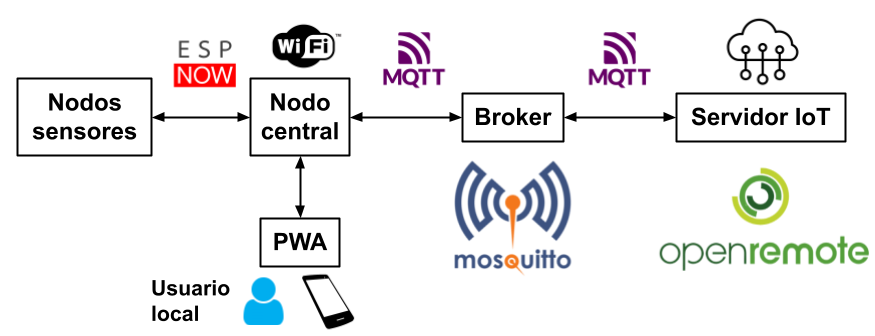
\includegraphics[width=1\textwidth]{./Figures/arq_sistema.png}
\caption{Esquema del sistema.}
\label{fig:arqSistema}
\end{figure}

En esta sección se describen los principales módulos que conforman el sistema, detallando su función y cómo interactúan entre sí.

\subsection{Nodos sensores} 

Están conformados por un módulo ESP32-C3 y un sensor. Esta es la capa de percepción, ya que los nodos son responsables de captar la información del entorno. Los datos recopilados son enviados al nodo central (gateway) a través del protocolo de comunicación ESP-NOW. En este contexto, también se incluye un módulo específico para gestionar los relés, cuyo estado puede ser consultado y modificado, por lo que se establece una \textit{comunicación bidireccional} con el \textit{gateway}. Sin embargo, en el caso de los sensores, la \textit{comunicación es unidireccional}, ya que solo envían datos.

\subsection{Nodo central}

Como se mencionó, este nodo se comunica con los sensores a través de ESP-NOW. Actúa como la capa de transporte, encargándose de transferir los datos capturados por la capa de percepción. Además, el \textit{gateway} integra una interfaz web embebida para visualizar los datos de los sensores y el estado de los relés. Esta interfaz está implementada utilizando un socket y, en caso de ausencia de conexión a internet, genera un “Access Point” (AP) local al cual el usuario puede conectarse para monitorear el estado del invernadero. El nodo central se conecta a internet mediante Wi-Fi para enviar los datos a un \textit{broker} MQTT (Mosquitto), empleando certificados TLS para asegurar la transmisión.

\subsection{Servidor IoT}

Este componente corresponde a la capa de procesamiento, donde se almacenan, analizan y gestionan los datos enviados desde el nodo central. Para esta función, se utilizará \textit{OpenRemote} como plataforma de servidor IoT, la cual facilita la integración de dispositivos y la gestión de datos. El servidor se conecta al \textit{broker} MQTT para recibir la información de los sensores y los relés.
Además de almacenar y visualizar los datos en tiempo real, el servidor permite generar informes, configurar alertas y ejecutar acciones automatizadas basadas en reglas predefinidas, como la activación de relés o notificaciones ante condiciones anómalas.



%----------------------------------------------------------------------------------------
\section{Desarrollo del firmware}

El \textit{firmware} del trabajo fue desarrollado utilizando el lenguaje de programación \textit{Python}, específicamente bajo el \textit{framework MicroPython}. Para su implementación, se empleó el entorno de desarrollo Visual Studio Code, que facilitó la edición y depuración del código.

En esta sección se presentan los diagramas de flujo que describen los procesos clave de los nodos sensores, el módulo de relés y el nodo central. Estos diagramas ilustran la lógica implementada en el \textit{firmware} y cómo se gestiona la comunicación eficiente entre sensores, actuadores, la interfaz web y el servidor IoT.

\subsection{Nodos sensores y módulo relés}

\subsubsection{Nodos sensores}

En la figura \ref{fig:flujoSensor} se presenta el diagrama de flujo de los nodos sensores. 

Cada sensor tendrá un script personalizado, ya que son diferentes entre sí, lo que implica que la forma de obtener las lecturas de los datos variará en cada caso. Sin embargo, el procedimiento para enviar los datos será el mismo para todos.

Primero, se inicializa y configura ESP-NOW para enviar mensajes en modo \textit{broadcast} (difusión) a todos los dispositivos cercanos, sin la necesidad de conocer sus direcciones MAC individuales
A continuación, el nodo busca el canal en el que se encuentra el \textit{gateway}. Una vez encontrado, se envía un mensaje de verificación para confirmar que el canal es el correcto. Si no se recibe respuesta, el nodo se reinicia, comenzando el proceso nuevamente.

Cuando el canal es verificado, se toma la lectura de los datos del sensor y se envía esta información al \textit{gateway} vía ESP-NOW, de forma encriptada, utilizando una librería específica de \textit{MicroPython} llamada \textit{cryptolib} \citep{docsmpy}.

Una vez que la información ha sido enviada, el dispositivo entra en \textit{modo DeepSleep} (sueño profundo) durante un tiempo determinado, con el fin de ahorrar energía. Al despertar, el módulo se reinicia como si hubiese sido encendido nuevamente.

\begin{figure}[H]
\centering 
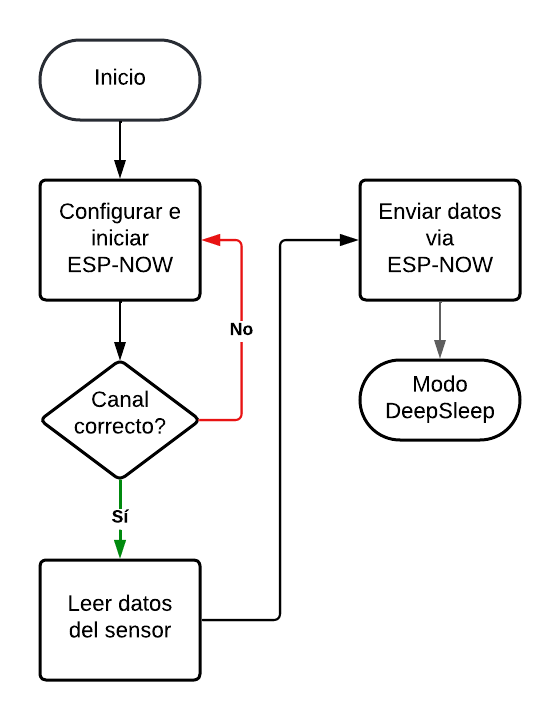
\includegraphics[width=0.5\textwidth]{./Figures/flujo_nodo_sensor.png}
\caption{Diagrama de flujo de los nodos sensores.}
\label{fig:flujoSensor}
\end{figure}

\subsubsection{Módulo relés}

El nodo encargado de los relés sigue un funcionamiento similar al de los nodos sensores en cuanto a la configuración inicial de ESP-NOW, por lo que no es necesario volver a detallar ese proceso. La principal diferencia radica en que, en lugar de tomar lecturas de un sensor, este nodo inicializa los relés y envía el estado en el que se encuentran al \textit{gateway}.

Una vez enviados los estados, el nodo queda a la espera de recibir instrucciones para modificar alguno de los relés. Si se recibe una solicitud para cambiar el estado de uno o más relés, el nodo ejecuta el cambio y, a continuación, envía nuevamente la información actualizada al \textit{gateway}.
Al igual que en los nodos sensores, la información se envía de forma encriptada para garantizar la seguridad de los datos transmitidos. De la misma manera, cualquier información que llega al nodo, como instrucciones para cambiar el estado de los relés, es desencriptada antes de ser procesada.

Este nodo no entra en \textit{modo DeepSleep}, ya que es necesario garantizar que los relés respondan de manera inmediata a cualquier instrucción de control que pueda recibirse.

En la figura \ref{fig:flujoRele} se puede observar el diagrama de flujo del módulo relés. 

\begin{figure}[H]
\centering 
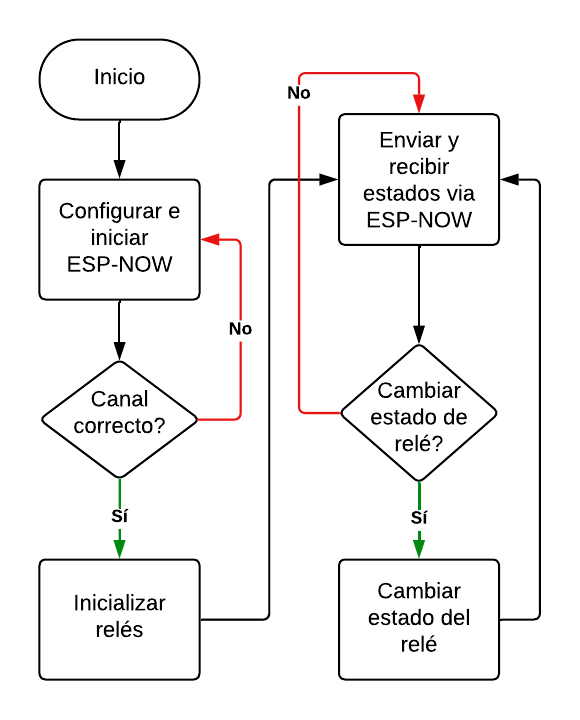
\includegraphics[width=0.5\textwidth]{./Figures/flujo_rele.png}
\caption{Diagrama de flujo del módulo relés.}
\label{fig:flujoRele}
\end{figure}

\subsection{Nodo Central}

El \textit{gateway} puede iniciar en dos modos diferentes: \textit{Modo Cliente} (CL) o \textit{Modo Access Point} (AP), dependiendo de la configuración cargada en el dispositivo. Una vez determinado el modo de operación, se configura e inicia la comunicación ESP-NOW en \textit{modo de difusión}.

\begin{itemize}
	\item Modo AP: en este caso, el \textit{gateway} actúa como un punto de acceso local, lo que significa que no está conectado a internet. Se inicia el servidor HTTP para proporcionar una interfaz web accesible a través de una red local, permitiendo al usuario monitorear y gestionar el sistema directamente sin necesidad de conexión externa.
	\item Modo CL: al iniciar en este modo significa que está conectado a internet a través de una red Wi-Fi. Se establece una conexión segura con un \textit{broker} MQTT. Para ello, se utilizan un nombre de usuario, una contraseña y certificados TLS para asegurar la comunicación. Además, el gateway se suscribe a un tópico específico del \textit{broker} MQTT, lo que le permite recibir mensajes relacionados con los sensores. Por último se inicia el servidor HTTP, lo que permite el acceso a la interfaz web embebida para monitorear y gestionar el sistema desde cualquier lugar con acceso a internet.
\end{itemize}

En la figura \ref{fig:flujoCentral} se puede observar el diagrama de flujo general del nodo central. 

\begin{figure}[H]
\centering 
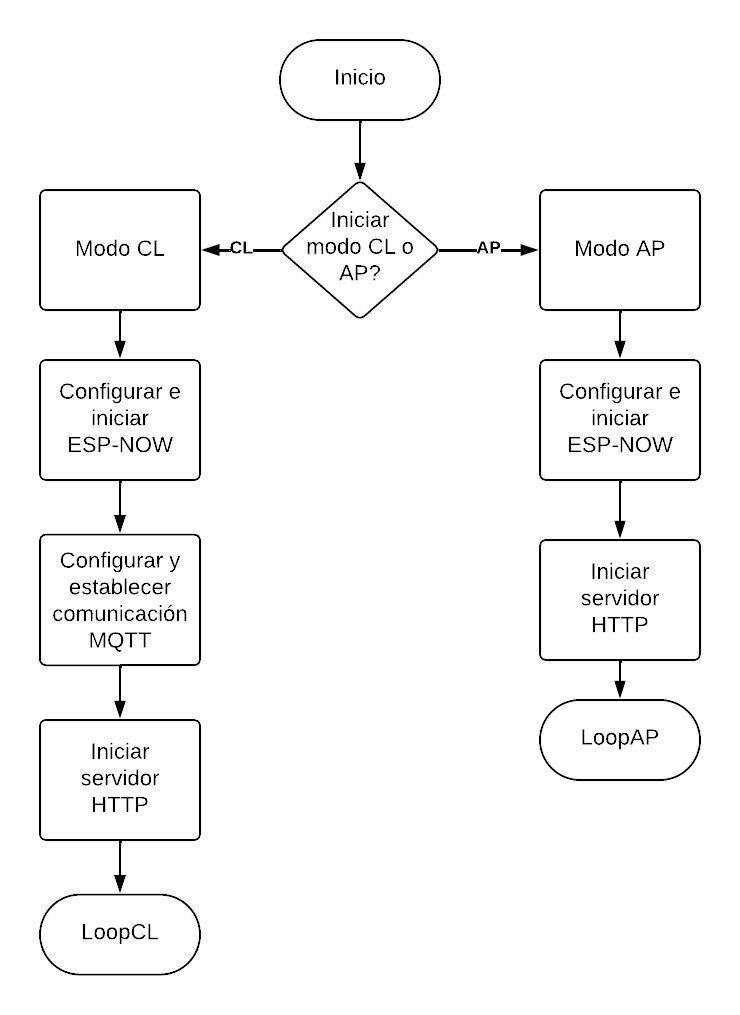
\includegraphics[width=0.7\textwidth]{./Figures/flujo_central.png}
\caption{Diagrama de flujo del nodo central.}
\label{fig:flujoCentral}
\end{figure}

\subsubsection{Loop AP}

En la figura \ref{fig:flujoAP} se puede observar el diagrama de flujo del loopAP. 

Una vez que el \textit{gateway} se ha iniciado en Modo AP y se ha configurado correctamente la comunicación ESP-NOW, entra en un bucle continuo de monitoreo y control, conocido como LoopAP. En este modo el \textit{gateway} realiza las siguientes acciones:

\begin{itemize}
	\item Monitoreo de nodos: el \textit{gateway} espera recibir datos de los nodos sensores y del módulo de relés a través de ESP-NOW. Al recibir información, ya sea de sensores o del estado de los relés, estos datos se envían y muestran en la PWA en tiempo real.
	\item Verificación de cambios en la PWA: si no se recibe información desde los nodos, el \textit{gateway} revisa si hubo un cambio en el estado de los relés en la PWA. Si detecta un cambio, envía la actualización al nodo correspondiente mediante ESP-NOW.
	\item Reinicio del ciclo: luego de procesar cualquier evento, el \textit{gateway} regresa al inicio del ciclo, quedando en espera de nuevos datos o cambios.
\end{itemize}


\begin{figure}[H]
\centering 
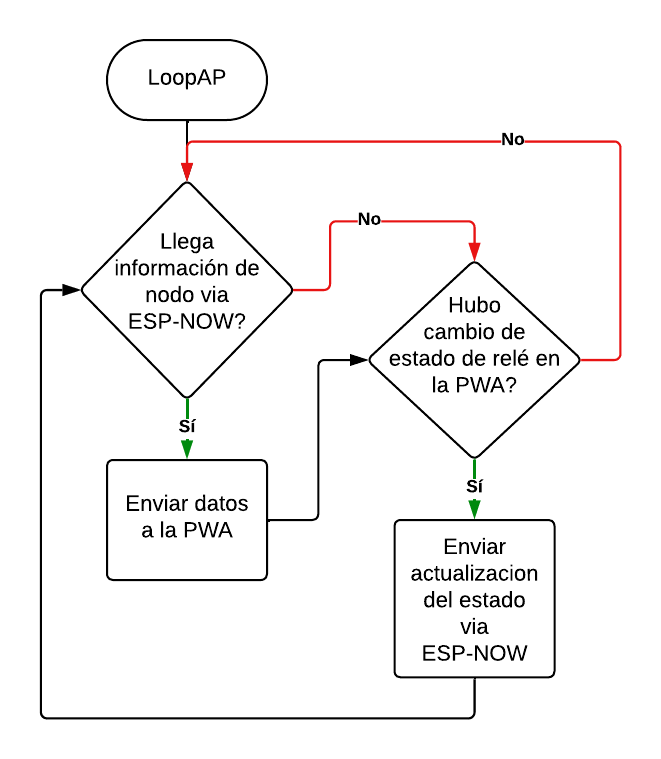
\includegraphics[width=0.5\textwidth]{./Figures/flujo_ap.png}
\caption{Diagrama de flujo del loop AP.}
\label{fig:flujoAP}
\end{figure}

\subsubsection{Loop CL}

En este modo, los datos de los sensores no solo se muestran localmente en la PWA, sino que también se publican en el \textit{broker} MQTT, lo que permite que sean almacenados y procesados remotamente. Esto garantiza una mayor capacidad de monitoreo y análisis.
Otra diferencia importante es la sincronización con el servidor IoT. Mientras que en el LoopAP los cambios en el estado de los relés solo se controlan desde la PWA, en el LoopCL también se monitorea si el estado de los relés ha sido modificado desde el servidor IoT. Esto posibilita la gestión remota de los dispositivos, permitiendo que el usuario controle y supervise el invernadero desde cualquier lugar con acceso a internet, una funcionalidad que no está disponible en el modo AP.

En la figura \ref{fig:flujoAP} se presenta el diagrama de flujo del loopCL. 

\begin{figure}[H]
\centering 
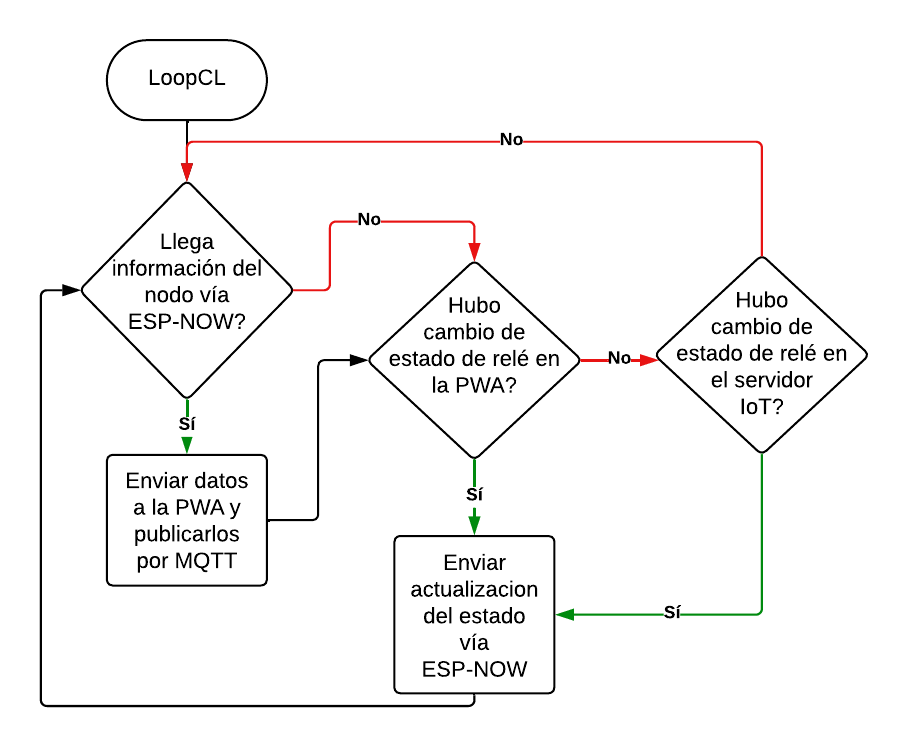
\includegraphics[width=0.6\textwidth]{./Figures/flujo_cl.png}
\caption{Diagrama de flujo del loop CL.}
\label{fig:flujoCL}
\end{figure}

%----------------------------------------------------------------------------------------
\section{Desarrollo de la aplicacion web progresiva}

%----------------------------------------------------------------------------------------
\section{Implementación del servidor IoT}

%----------------------------------------------------------------------------------------
\section{Despliegue del sistema}




	% Chapter Template

\chapter{Ensayos y resultados} % Main chapter title

\label{Chapter4} % Change X to a consecutive number; for referencing this chapter elsewhere, use \ref{ChapterX}

%----------------------------------------------------------------------------------------
%	SECTION 1
%----------------------------------------------------------------------------------------

\section{Pruebas funcionales del hardware}
\label{sec:pruebasHW}

La idea de esta sección es explicar cómo se hicieron los ensayos, qué resultados se obtuvieron y analizarlos.
 
	% Chapter Template

\chapter{Conclusiones} % Main chapter title

\label{Chapter5} % Change X to a consecutive number; for referencing this chapter elsewhere, use \ref{ChapterX}


%----------------------------------------------------------------------------------------

%----------------------------------------------------------------------------------------
%	SECTION 1
%----------------------------------------------------------------------------------------

\section{Conclusiones del trabajo realizado}

En la presente memoria de tesis se ha documentado el Trabajo Final para la obtención del grado de \degreename.  

Se obtuvo un \textit{firmware} que permite controlar un acuario en forma remota mediante una interfaz web embebida en la plataforma CIAA-NXP. Se aplicaron simplificaciones al modelo de acuario, principalmente debido a las restricciones de tiempo establecidas para la finalización del trabajo y a la ejecución de acciones de contingencia de riesgos identificados al comienzo de la planificación del trabajo, a saber:

\begin{itemize}
	\item Riesgo: No contar con un subsidio para la adquisición de sensores y actuadores de acuario.
	\item Riesgo: No disponer de una CIAA-NXP a tiempo para el comienzo del proyecto.
	\item Contingencia:  Simular sensores y actuadores del modelo de acuario.
\end{itemize}

Con las mencionadas simplificaciones se obtuvo una ``planta piloto'' que permitió avanzar en el desarrollo del \textit{firmware} de control y cumplir con los requerimientos de tiempo de finalización.

Se pudo integrar el \textit{stack} TCP/IP lwIP con el RTOS freeRTOS al \textit{firmware} de control sobre la base de un \textit{port} desarrollado por NXP, fabricante del microcontrolador LPC4337.

\medskip

Durante el desarrollo de este Trabajo Final se aplicaron conocimientos adquiridos a lo largo de la Carrera de Especialización en Sistemas Embebidos. Si bien el conjunto total de asignaturas cursadas aportaron conocimientos necesarios para la práctica profesional en el área de los Sistemas Embebidos, se quiere dejar constancia en particular, de las asignaturas con mayor relevancia para el trabajo presentado.

\begin{itemize}
\item
\textbf{Arquitectura de microprocesadores}. Resultó necesario tener conocimientos sobre la Arquitectura ARM Cortex M para la programación de la plataforma CIAA-NXP y el uso de los periféricos.

\item
\textbf{Programación de microprocesadores}. Se utilizaron buenas prácticas de programación de Lenguaje C para microcontroladores y periféricos, aprendidas en esta asignatura. Se empleó un formato de código consistente: comentarios en las declaraciones de funciones y partes importantes del código, constantes en mayúsculas, \textit{camelCase} para poner nombres significativos a funciones y variables. Se utilizaron APIs\footnote{\textit{Application Program Interface}} para abstraer distintas capas del código. Se obtuvo un código más legible y reutilizable.

\item
\textbf{Ingeniería de Software en Sistemas Embebidos}. Se utilizaron técnicas provenientes de la Ingeniería de Software. Siempre que fue posible se utilizó un método sistemático e iterativo de desarrollo pensando en el ciclo de vida del \textit{software}. Se hizo uso extensivo de Git como sistema de control de versiones del software.  Asimismo, se aplicaron metodologías de ensayo de \textit{software} aprendidas en esta asignatura.

\item
\textbf{Gestión de Proyectos en Ingeniería}. Resultó de gran utilidad elaborar un Plan de Proyecto para organizar el Trabajo Final.  Parte del material elaborado en esta asignatura como la planificación y el desglose de tareas se pueden encontrar en la presente memoria, en el capítulo \ref{Chapter2}.

\item
\textbf{Sistemas Operativos de Tiempo Real (I y II)}. Se aplicaron los conocimientos adquiridos sobre freeRTOS respecto a tareas, cambios de contexto y semáforos entre otros.  Asimismo, se utilizaron herramientas de desarrollo propias de freeRTOS para medir el uso de las pilas de las tareas creadas y optimizar el uso de la memoria.

\item 
\textbf{Protocolos de Comunicación}. Se aplicaron ampliamente los conocimientos obtenidos en el área de Ethernet. En particular, resultó útil el material sobre el \textit{stack} TCP/IP lwIP.

\item
\textbf{Diseño de Sistemas Críticos}. Siempre que fue posible se utilizaron técnicas de programación defensiva para que el comportamiento del \textit{firmware} resulte lo más predecible posible.  Se buscó obtener un sistema de control que no falle en primer lugar, y que si lo hace, falle en forma segura evitando daños tanto a los seres vivos dentro y fuera del acuario como a la propiedad.
\end{itemize}



\medskip

\noindent Asimismo, durante el desarrollo del trabajo final se adquirieron conocimientos en las áreas de:

\begin{itemize}
	\item Programación en lenguaje HTML5.
	\item Programación en lenguaje JavaScript.  
	\item Utilización de \textit{linker scripts} para el entorno de desarrollo LPCXpresso.
\end{itemize}


\medskip

Por lo tanto, se concluye que los objetivos planteados al comienzo del trabajo han sido alcanzados satisfactoriamente, habiéndose cumplido con los criterios de aceptación del sistema final y además, se han obtenido conocimientos valiosos para la formación profesional del autor.

%----------------------------------------------------------------------------------------
%	SECTION 2
%----------------------------------------------------------------------------------------
\clearpage
\section{Trabajo futuro}

Se considera oportuno identificar las líneas de trabajo futuro para dar continuidad al esfuerzo invertido.  Se listan a continuación las principales.

\begin{itemize}
	\item Trabajar con una planta piloto real, con sensores y actuadores de acuario.  Caracterizar la dinámica del entorno real y ajustar la lógica de control si fuera necesario.
	\vspace{5px}
	\item Escalar el \textit{firmware} desarrollado para obtener un \textit{framework} que posibilite cambiar el dominio de aplicación a otras áreas de control donde el modelo de ``medir, alertar y actuar'' aplique.
	\vspace{5px}
	\item Permitir la introducción de nuevos sensores y actuadores debidamente parametrizados mediante la interfaz de usuario.
	\vspace{5px}
	\item Mejorar la portabilidad de la interfaz web utilizando técnicas de RWD (\textit{Responsive Web Design}) para que permita su correcta visualización en distintos dispositivos, navegadores y resoluciones de pantalla.
\end{itemize}






 
\end{verbatim}

Los apéndices también deben escribirse en archivos .tex separados, que se deben ubicar dentro de la carpeta \emph{Appendices}. Los apéndices vienen comentados por defecto con el caracter \code{\%} y para incluirlos simplemente se debe eliminar dicho caracter.

Finalmente, se encuentra el código para incluir la bibliografía en el documento final.  Este código tampoco debe modificarse. La metodología para trabajar las referencias bibliográficas se desarrolla en la sección \ref{sec:biblio}.
%----------------------------------------------------------------------------------------

\section{Bibliografía}
\label{sec:biblio}

Las opciones de formato de la bibliografía se controlan a través del paquete de latex \option{biblatex} que se incluye en la memoria en el archivo memoria.tex.  Estas opciones determinan cómo se generan las citas bibliográficas en el cuerpo del documento y cómo se genera la biblografía al final de la memoria.

En el preámbulo se puede encontrar el código que incluye el paquete biblatex, que no requiere ninguna modificación del usuario de la plantilla, y que contiene las siguientes opciones:

\begin{lstlisting}
\usepackage[backend=bibtex,
	natbib=true, 
	style=numeric, 
	sorting=none]
{biblatex}
\end{lstlisting}

En el archivo \file{reference.bib} se encuentran las referencias bibliográficas que se pueden citar en el documento.  Para incorporar una nueva cita al documento lo primero es agregarla en este archivo con todos los campos necesario.  Todas las entradas bibliográficas comienzan con $@$ y una palabra que define el formato de la entrada.  Para cada formato existen campos obligatorios que deben completarse. No importa el orden en que las entradas estén definidas en el archivo .bib.  Tampoco es importante el orden en que estén definidos los campos de una entrada bibliográfica. A continuación se muestran algunos ejemplos:

\begin{lstlisting}
@ARTICLE{ARTICLE:1,
    AUTHOR="John Doe",
    TITLE="Title",
    JOURNAL="Journal",
    YEAR="2017",
}
\end{lstlisting}


\begin{lstlisting}
@BOOK{BOOK:1,
    AUTHOR="John Doe",
    TITLE="The Book without Title",
    PUBLISHER="Dummy Publisher",
    YEAR="2100",
}
\end{lstlisting}


\begin{lstlisting}
@INBOOK{BOOK:2,
    AUTHOR="John Doe",
    TITLE="The Book without Title",
    PUBLISHER="Dummy Publisher",
    YEAR="2100",
    PAGES="100-200",
}
\end{lstlisting}


\begin{lstlisting}
@MISC{WEBSITE:1,
    HOWPUBLISHED = "\url{http://example.com}",
    AUTHOR = "Intel",
    TITLE = "Example Website",
    MONTH = "12",
    YEAR = "1988",
    URLDATE = {2012-11-26}
}
\end{lstlisting}

Se debe notar que los nombres \emph{ARTICLE:1}, \emph{BOOK:1}, \emph{BOOK:2} y \emph{WEBSITE:1} son nombres de fantasía que le sirve al autor del documento para indentificar la entrada. En este sentido, se podrían reemplazar por cualquier otro nombre.  Tampoco es necesario poner : seguido de un número, en los ejemplos sólo se incluye como un posible estilo para identificar las entradas.

La entradas se citan en el documento con el comando: 

\begin{verbatim}
\citep{nombre_de_la_entrada}
\end{verbatim}

Y cuando se usan, se muestran así: \citep{ARTICLE:1}, \citep{BOOK:1}, \citep{BOOK:2}, \citep{WEBSITE:1}.  Notar cómo se conforma la sección Bibliografía al final del documento. 

	\chapter{Introducción Específica} % Main chapter title

\label{Chapter2}

%----------------------------------------------------------------------------------------
%	SECTION 1
%----------------------------------------------------------------------------------------

\section{Título de la sección con este uso de las mayúsculas}
\label{sec:ejemplo}
La idea de esta sección es presentar el tema de modo que cualquier persona que no conoce el tema pueda entender de qué se trata y por qué es importante realizar este trabajo y cuál es su impacto.

Si en el texto se hace alusión a diferentes partes del trabajo referirse a ellas como Capítulo, Sección o subsección según corresponda. Por ejemplo: ``En el Capítulo \ref{Chapter1} se explica tal cosa'', o ``En la Sección \ref{sec:ejemplo} se presenta lo que sea'', o ``En la la subsección \ref{subsec:ejemplo} se discute otra cosa''.

Entre párrafos sucesivos dejar un espacio, como el que se observa entre este párrafo y el anterior. Pero las oraciones de un mismo párrafo van en forma consecutiva, como se observa acá. Luego, cuando se quiere poner una lista tabulada se hace así:

\begin{itemize}
	\item Este es el primer elemento de la lista.
	\item Este es el segundo elemento de la lista.
\end{itemize}

Notar el uso de las mayúsculas y el punto al final de cada elemento.
Si se desea poner una lista numerada el formato es este:
\begin{enumerate}
	\item Este es el primer elemento de la lista.
	\item Este es el segundo elemento de la lista.
\end{enumerate}

Notar el uso de las mayúsculas y el punto al final de cada elemento.

\subsection{Este es el título de una subsección}
\label{subsec:ejemplo}

Se recomienda no utilizar \textbf{texto en negritas} en ningún párrafo, ni tampoco \underline{texto subrayado}. En cambio sí se sugiere utilizar \textit{texto en cursiva} donde se considere apropiado.

Se sugiere que la escritura sea impersonal. Por ejemplo, no utilizar ``el diseño del firmware lo hice de acuerdo con tal principio'', sino ``el firmware fue diseñado utilizando tal principio''. En lo posible hablar en tiempo pasado, ya que la memoria describe un trabajo que ya fue realizado.

Se recomienda no utilizar una sección de glosario sino colocar la descripción de las abreviaturas como parte del mismo cuerpo del texto. Por ejemplo, RTOS (\textit{Real Time Operating System}, Sistema Operativo de Tiempo Real) o en caso de considerarlo apropiado mediante notas a pie de página.

Si se desea indicar alguna página web utilizar el siguiente formato de referencias bibliográficas, dónde las referencias se detallan en la sección de bibliografía de la memoria,utilizado el formato establecido por IEEE en [1]. Por ejemplo, ``el presente trabajo se basa en la plataforma EDU-CIAA-NXP, la cual se describe en detalle en [2]''. 
 
	\chapter{Diseño e implementación} % Main chapter title

En este capítulo se van a describir las soluciones planteadas al problema resuelto en este trabajo.

%----------------------------------------------------------------------------------------
%	SECTION 1
%----------------------------------------------------------------------------------------
\section{Arquitectura del sistema}

En la figura \ref{fig:arqSistema} se puede observar un esquema simple del sistema, donde se tiene:

\begin{itemize}
	\item Nodos sensores.
	\item Nodo Central.
	\item Aplicacion web progresiva.
	\item Broker.
	\item Servidor IoT.
\end{itemize}

\begin{figure}[H]
\centering 
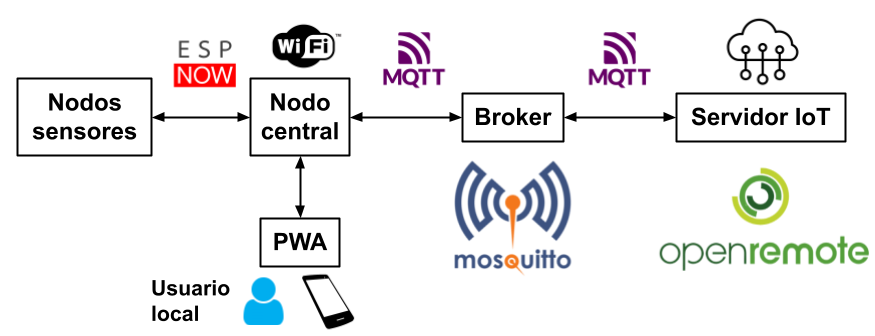
\includegraphics[width=1\textwidth]{./Figures/arq_sistema.png}
\caption{Esquema del sistema.}
\label{fig:arqSistema}
\end{figure}

En esta sección se describen los principales módulos que conforman el sistema, detallando su función y cómo interactúan entre sí.

\subsection{Nodos sensores} 

Están conformados por un módulo ESP32-C3 y un sensor. Esta es la capa de percepción, ya que los nodos son responsables de captar la información del entorno. Los datos recopilados son enviados al nodo central (gateway) a través del protocolo de comunicación ESP-NOW. En este contexto, también se incluye un módulo específico para gestionar los relés, cuyo estado puede ser consultado y modificado, por lo que se establece una \textit{comunicación bidireccional} con el \textit{gateway}. Sin embargo, en el caso de los sensores, la \textit{comunicación es unidireccional}, ya que solo envían datos.

\subsection{Nodo central}

Como se mencionó, este nodo se comunica con los sensores a través de ESP-NOW. Actúa como la capa de transporte, encargándose de transferir los datos capturados por la capa de percepción. Además, el \textit{gateway} integra una interfaz web embebida para visualizar los datos de los sensores y el estado de los relés. Esta interfaz está implementada utilizando un socket y, en caso de ausencia de conexión a internet, genera un “Access Point” (AP) local al cual el usuario puede conectarse para monitorear el estado del invernadero. El nodo central se conecta a internet mediante Wi-Fi para enviar los datos a un \textit{broker} MQTT (Mosquitto), empleando certificados TLS para asegurar la transmisión.

\subsection{Servidor IoT}

Este componente corresponde a la capa de procesamiento, donde se almacenan, analizan y gestionan los datos enviados desde el nodo central. Para esta función, se utilizará \textit{OpenRemote} como plataforma de servidor IoT, la cual facilita la integración de dispositivos y la gestión de datos. El servidor se conecta al \textit{broker} MQTT para recibir la información de los sensores y los relés.
Además de almacenar y visualizar los datos en tiempo real, el servidor permite generar informes, configurar alertas y ejecutar acciones automatizadas basadas en reglas predefinidas, como la activación de relés o notificaciones ante condiciones anómalas.



%----------------------------------------------------------------------------------------
\section{Desarrollo del firmware}

El \textit{firmware} del trabajo fue desarrollado utilizando el lenguaje de programación \textit{Python}, específicamente bajo el \textit{framework MicroPython}. Para su implementación, se empleó el entorno de desarrollo Visual Studio Code, que facilitó la edición y depuración del código.

En esta sección se presentan los diagramas de flujo que describen los procesos clave de los nodos sensores, el módulo de relés y el nodo central. Estos diagramas ilustran la lógica implementada en el \textit{firmware} y cómo se gestiona la comunicación eficiente entre sensores, actuadores, la interfaz web y el servidor IoT.

\subsection{Nodos sensores y módulo relés}

\subsubsection{Nodos sensores}

En la figura \ref{fig:flujoSensor} se presenta el diagrama de flujo de los nodos sensores. 

Cada sensor tendrá un script personalizado, ya que son diferentes entre sí, lo que implica que la forma de obtener las lecturas de los datos variará en cada caso. Sin embargo, el procedimiento para enviar los datos será el mismo para todos.

Primero, se inicializa y configura ESP-NOW para enviar mensajes en modo \textit{broadcast} (difusión) a todos los dispositivos cercanos, sin la necesidad de conocer sus direcciones MAC individuales
A continuación, el nodo busca el canal en el que se encuentra el \textit{gateway}. Una vez encontrado, se envía un mensaje de verificación para confirmar que el canal es el correcto. Si no se recibe respuesta, el nodo se reinicia, comenzando el proceso nuevamente.

Cuando el canal es verificado, se toma la lectura de los datos del sensor y se envía esta información al \textit{gateway} vía ESP-NOW, de forma encriptada, utilizando una librería específica de \textit{MicroPython} llamada \textit{cryptolib} \citep{docsmpy}.

Una vez que la información ha sido enviada, el dispositivo entra en \textit{modo DeepSleep} (sueño profundo) durante un tiempo determinado, con el fin de ahorrar energía. Al despertar, el módulo se reinicia como si hubiese sido encendido nuevamente.

\begin{figure}[H]
\centering 
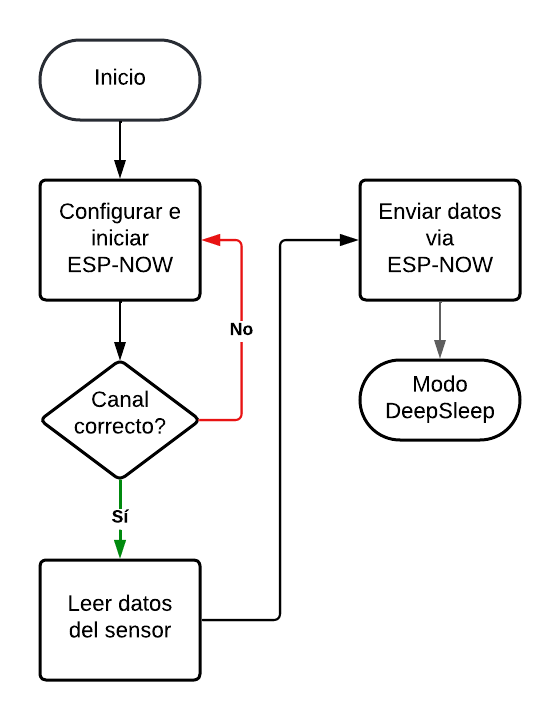
\includegraphics[width=0.5\textwidth]{./Figures/flujo_nodo_sensor.png}
\caption{Diagrama de flujo de los nodos sensores.}
\label{fig:flujoSensor}
\end{figure}

\subsubsection{Módulo relés}

El nodo encargado de los relés sigue un funcionamiento similar al de los nodos sensores en cuanto a la configuración inicial de ESP-NOW, por lo que no es necesario volver a detallar ese proceso. La principal diferencia radica en que, en lugar de tomar lecturas de un sensor, este nodo inicializa los relés y envía el estado en el que se encuentran al \textit{gateway}.

Una vez enviados los estados, el nodo queda a la espera de recibir instrucciones para modificar alguno de los relés. Si se recibe una solicitud para cambiar el estado de uno o más relés, el nodo ejecuta el cambio y, a continuación, envía nuevamente la información actualizada al \textit{gateway}.
Al igual que en los nodos sensores, la información se envía de forma encriptada para garantizar la seguridad de los datos transmitidos. De la misma manera, cualquier información que llega al nodo, como instrucciones para cambiar el estado de los relés, es desencriptada antes de ser procesada.

Este nodo no entra en \textit{modo DeepSleep}, ya que es necesario garantizar que los relés respondan de manera inmediata a cualquier instrucción de control que pueda recibirse.

En la figura \ref{fig:flujoRele} se puede observar el diagrama de flujo del módulo relés. 

\begin{figure}[H]
\centering 
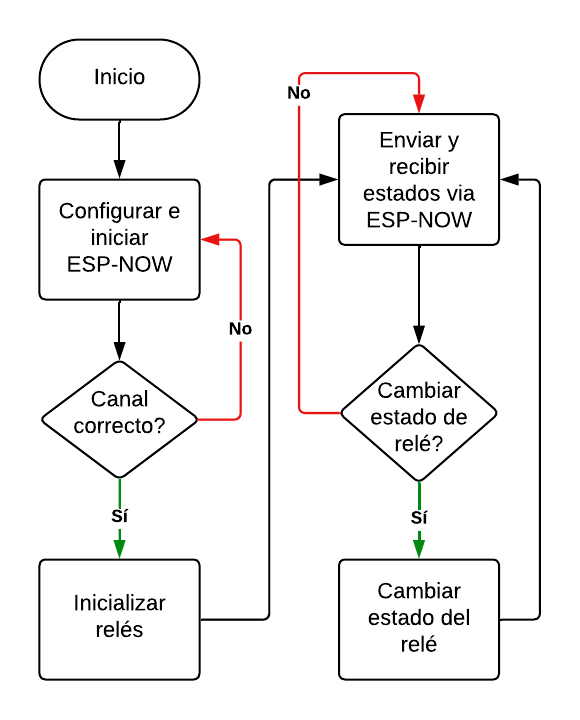
\includegraphics[width=0.5\textwidth]{./Figures/flujo_rele.png}
\caption{Diagrama de flujo del módulo relés.}
\label{fig:flujoRele}
\end{figure}

\subsection{Nodo Central}

El \textit{gateway} puede iniciar en dos modos diferentes: \textit{Modo Cliente} (CL) o \textit{Modo Access Point} (AP), dependiendo de la configuración cargada en el dispositivo. Una vez determinado el modo de operación, se configura e inicia la comunicación ESP-NOW en \textit{modo de difusión}.

\begin{itemize}
	\item Modo AP: en este caso, el \textit{gateway} actúa como un punto de acceso local, lo que significa que no está conectado a internet. Se inicia el servidor HTTP para proporcionar una interfaz web accesible a través de una red local, permitiendo al usuario monitorear y gestionar el sistema directamente sin necesidad de conexión externa.
	\item Modo CL: al iniciar en este modo significa que está conectado a internet a través de una red Wi-Fi. Se establece una conexión segura con un \textit{broker} MQTT. Para ello, se utilizan un nombre de usuario, una contraseña y certificados TLS para asegurar la comunicación. Además, el gateway se suscribe a un tópico específico del \textit{broker} MQTT, lo que le permite recibir mensajes relacionados con los sensores. Por último se inicia el servidor HTTP, lo que permite el acceso a la interfaz web embebida para monitorear y gestionar el sistema desde cualquier lugar con acceso a internet.
\end{itemize}

En la figura \ref{fig:flujoCentral} se puede observar el diagrama de flujo general del nodo central. 

\begin{figure}[H]
\centering 
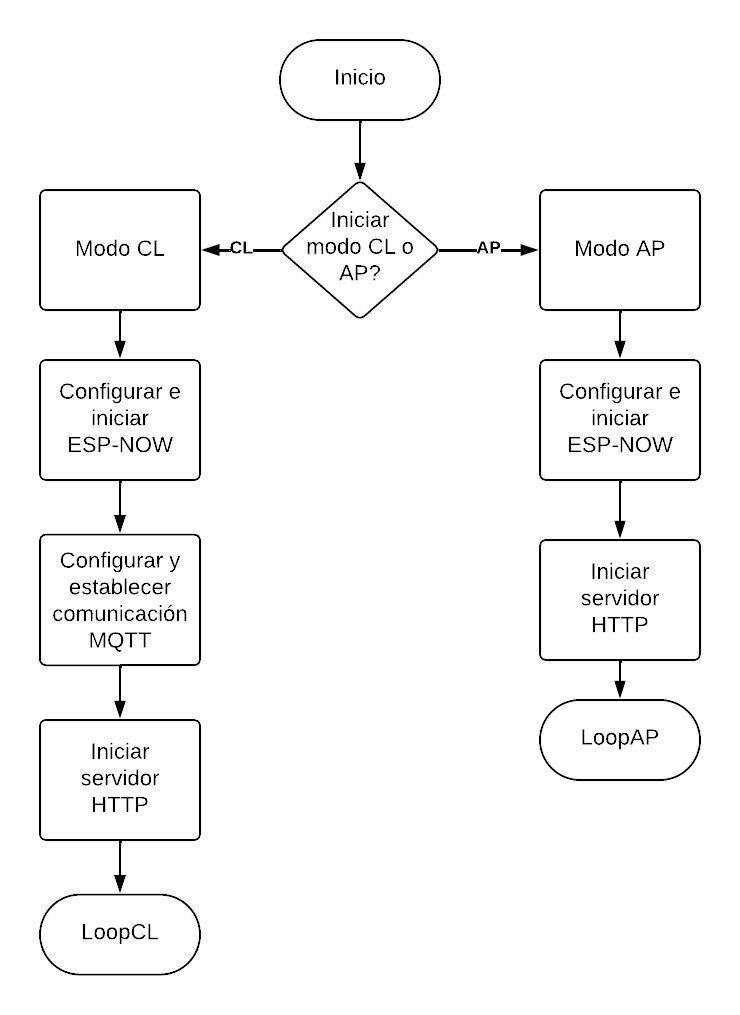
\includegraphics[width=0.7\textwidth]{./Figures/flujo_central.png}
\caption{Diagrama de flujo del nodo central.}
\label{fig:flujoCentral}
\end{figure}

\subsubsection{Loop AP}

En la figura \ref{fig:flujoAP} se puede observar el diagrama de flujo del loopAP. 

Una vez que el \textit{gateway} se ha iniciado en Modo AP y se ha configurado correctamente la comunicación ESP-NOW, entra en un bucle continuo de monitoreo y control, conocido como LoopAP. En este modo el \textit{gateway} realiza las siguientes acciones:

\begin{itemize}
	\item Monitoreo de nodos: el \textit{gateway} espera recibir datos de los nodos sensores y del módulo de relés a través de ESP-NOW. Al recibir información, ya sea de sensores o del estado de los relés, estos datos se envían y muestran en la PWA en tiempo real.
	\item Verificación de cambios en la PWA: si no se recibe información desde los nodos, el \textit{gateway} revisa si hubo un cambio en el estado de los relés en la PWA. Si detecta un cambio, envía la actualización al nodo correspondiente mediante ESP-NOW.
	\item Reinicio del ciclo: luego de procesar cualquier evento, el \textit{gateway} regresa al inicio del ciclo, quedando en espera de nuevos datos o cambios.
\end{itemize}


\begin{figure}[H]
\centering 
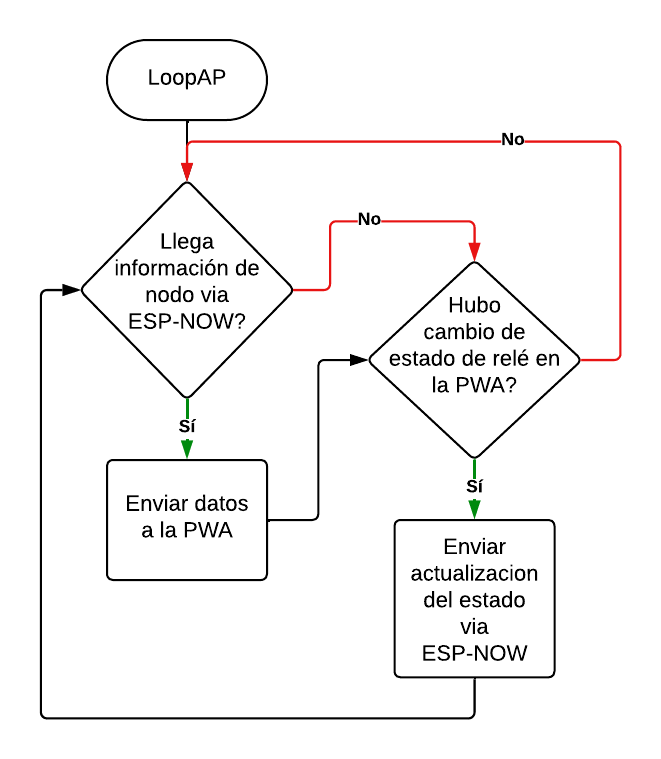
\includegraphics[width=0.5\textwidth]{./Figures/flujo_ap.png}
\caption{Diagrama de flujo del loop AP.}
\label{fig:flujoAP}
\end{figure}

\subsubsection{Loop CL}

En este modo, los datos de los sensores no solo se muestran localmente en la PWA, sino que también se publican en el \textit{broker} MQTT, lo que permite que sean almacenados y procesados remotamente. Esto garantiza una mayor capacidad de monitoreo y análisis.
Otra diferencia importante es la sincronización con el servidor IoT. Mientras que en el LoopAP los cambios en el estado de los relés solo se controlan desde la PWA, en el LoopCL también se monitorea si el estado de los relés ha sido modificado desde el servidor IoT. Esto posibilita la gestión remota de los dispositivos, permitiendo que el usuario controle y supervise el invernadero desde cualquier lugar con acceso a internet, una funcionalidad que no está disponible en el modo AP.

En la figura \ref{fig:flujoAP} se presenta el diagrama de flujo del loopCL. 

\begin{figure}[H]
\centering 
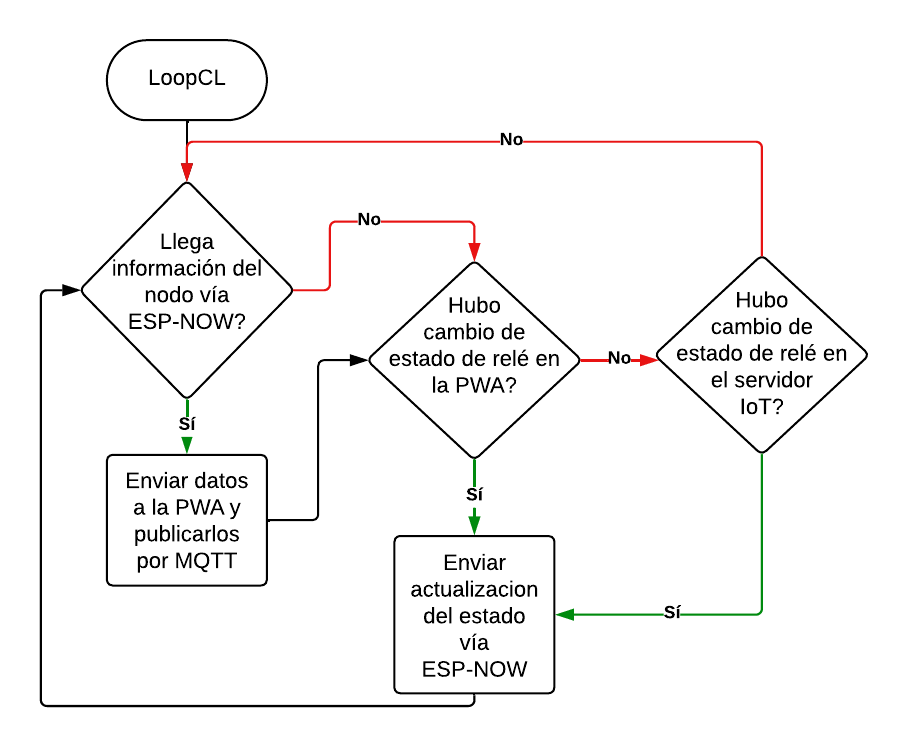
\includegraphics[width=0.6\textwidth]{./Figures/flujo_cl.png}
\caption{Diagrama de flujo del loop CL.}
\label{fig:flujoCL}
\end{figure}

%----------------------------------------------------------------------------------------
\section{Desarrollo de la aplicacion web progresiva}

%----------------------------------------------------------------------------------------
\section{Implementación del servidor IoT}

%----------------------------------------------------------------------------------------
\section{Despliegue del sistema}




	% Chapter Template

\chapter{Ensayos y resultados} % Main chapter title

\label{Chapter4} % Change X to a consecutive number; for referencing this chapter elsewhere, use \ref{ChapterX}

%----------------------------------------------------------------------------------------
%	SECTION 1
%----------------------------------------------------------------------------------------

\section{Pruebas funcionales del hardware}
\label{sec:pruebasHW}

La idea de esta sección es explicar cómo se hicieron los ensayos, qué resultados se obtuvieron y analizarlos.
 
	% Chapter Template

\chapter{Conclusiones} % Main chapter title

\label{Chapter5} % Change X to a consecutive number; for referencing this chapter elsewhere, use \ref{ChapterX}


%----------------------------------------------------------------------------------------

%----------------------------------------------------------------------------------------
%	SECTION 1
%----------------------------------------------------------------------------------------

\section{Conclusiones del trabajo realizado}

En la presente memoria de tesis se ha documentado el Trabajo Final para la obtención del grado de \degreename.  

Se obtuvo un \textit{firmware} que permite controlar un acuario en forma remota mediante una interfaz web embebida en la plataforma CIAA-NXP. Se aplicaron simplificaciones al modelo de acuario, principalmente debido a las restricciones de tiempo establecidas para la finalización del trabajo y a la ejecución de acciones de contingencia de riesgos identificados al comienzo de la planificación del trabajo, a saber:

\begin{itemize}
	\item Riesgo: No contar con un subsidio para la adquisición de sensores y actuadores de acuario.
	\item Riesgo: No disponer de una CIAA-NXP a tiempo para el comienzo del proyecto.
	\item Contingencia:  Simular sensores y actuadores del modelo de acuario.
\end{itemize}

Con las mencionadas simplificaciones se obtuvo una ``planta piloto'' que permitió avanzar en el desarrollo del \textit{firmware} de control y cumplir con los requerimientos de tiempo de finalización.

Se pudo integrar el \textit{stack} TCP/IP lwIP con el RTOS freeRTOS al \textit{firmware} de control sobre la base de un \textit{port} desarrollado por NXP, fabricante del microcontrolador LPC4337.

\medskip

Durante el desarrollo de este Trabajo Final se aplicaron conocimientos adquiridos a lo largo de la Carrera de Especialización en Sistemas Embebidos. Si bien el conjunto total de asignaturas cursadas aportaron conocimientos necesarios para la práctica profesional en el área de los Sistemas Embebidos, se quiere dejar constancia en particular, de las asignaturas con mayor relevancia para el trabajo presentado.

\begin{itemize}
\item
\textbf{Arquitectura de microprocesadores}. Resultó necesario tener conocimientos sobre la Arquitectura ARM Cortex M para la programación de la plataforma CIAA-NXP y el uso de los periféricos.

\item
\textbf{Programación de microprocesadores}. Se utilizaron buenas prácticas de programación de Lenguaje C para microcontroladores y periféricos, aprendidas en esta asignatura. Se empleó un formato de código consistente: comentarios en las declaraciones de funciones y partes importantes del código, constantes en mayúsculas, \textit{camelCase} para poner nombres significativos a funciones y variables. Se utilizaron APIs\footnote{\textit{Application Program Interface}} para abstraer distintas capas del código. Se obtuvo un código más legible y reutilizable.

\item
\textbf{Ingeniería de Software en Sistemas Embebidos}. Se utilizaron técnicas provenientes de la Ingeniería de Software. Siempre que fue posible se utilizó un método sistemático e iterativo de desarrollo pensando en el ciclo de vida del \textit{software}. Se hizo uso extensivo de Git como sistema de control de versiones del software.  Asimismo, se aplicaron metodologías de ensayo de \textit{software} aprendidas en esta asignatura.

\item
\textbf{Gestión de Proyectos en Ingeniería}. Resultó de gran utilidad elaborar un Plan de Proyecto para organizar el Trabajo Final.  Parte del material elaborado en esta asignatura como la planificación y el desglose de tareas se pueden encontrar en la presente memoria, en el capítulo \ref{Chapter2}.

\item
\textbf{Sistemas Operativos de Tiempo Real (I y II)}. Se aplicaron los conocimientos adquiridos sobre freeRTOS respecto a tareas, cambios de contexto y semáforos entre otros.  Asimismo, se utilizaron herramientas de desarrollo propias de freeRTOS para medir el uso de las pilas de las tareas creadas y optimizar el uso de la memoria.

\item 
\textbf{Protocolos de Comunicación}. Se aplicaron ampliamente los conocimientos obtenidos en el área de Ethernet. En particular, resultó útil el material sobre el \textit{stack} TCP/IP lwIP.

\item
\textbf{Diseño de Sistemas Críticos}. Siempre que fue posible se utilizaron técnicas de programación defensiva para que el comportamiento del \textit{firmware} resulte lo más predecible posible.  Se buscó obtener un sistema de control que no falle en primer lugar, y que si lo hace, falle en forma segura evitando daños tanto a los seres vivos dentro y fuera del acuario como a la propiedad.
\end{itemize}



\medskip

\noindent Asimismo, durante el desarrollo del trabajo final se adquirieron conocimientos en las áreas de:

\begin{itemize}
	\item Programación en lenguaje HTML5.
	\item Programación en lenguaje JavaScript.  
	\item Utilización de \textit{linker scripts} para el entorno de desarrollo LPCXpresso.
\end{itemize}


\medskip

Por lo tanto, se concluye que los objetivos planteados al comienzo del trabajo han sido alcanzados satisfactoriamente, habiéndose cumplido con los criterios de aceptación del sistema final y además, se han obtenido conocimientos valiosos para la formación profesional del autor.

%----------------------------------------------------------------------------------------
%	SECTION 2
%----------------------------------------------------------------------------------------
\clearpage
\section{Trabajo futuro}

Se considera oportuno identificar las líneas de trabajo futuro para dar continuidad al esfuerzo invertido.  Se listan a continuación las principales.

\begin{itemize}
	\item Trabajar con una planta piloto real, con sensores y actuadores de acuario.  Caracterizar la dinámica del entorno real y ajustar la lógica de control si fuera necesario.
	\vspace{5px}
	\item Escalar el \textit{firmware} desarrollado para obtener un \textit{framework} que posibilite cambiar el dominio de aplicación a otras áreas de control donde el modelo de ``medir, alertar y actuar'' aplique.
	\vspace{5px}
	\item Permitir la introducción de nuevos sensores y actuadores debidamente parametrizados mediante la interfaz de usuario.
	\vspace{5px}
	\item Mejorar la portabilidad de la interfaz web utilizando técnicas de RWD (\textit{Responsive Web Design}) para que permita su correcta visualización en distintos dispositivos, navegadores y resoluciones de pantalla.
\end{itemize}






 
\end{verbatim}

Los apéndices también deben escribirse en archivos .tex separados, que se deben ubicar dentro de la carpeta \emph{Appendices}. Los apéndices vienen comentados por defecto con el caracter \code{\%} y para incluirlos simplemente se debe eliminar dicho caracter.

Finalmente, se encuentra el código para incluir la bibliografía en el documento final.  Este código tampoco debe modificarse. La metodología para trabajar las referencias bibliográficas se desarrolla en la sección \ref{sec:biblio}.
%----------------------------------------------------------------------------------------

\section{Bibliografía}
\label{sec:biblio}

Las opciones de formato de la bibliografía se controlan a través del paquete de latex \option{biblatex} que se incluye en la memoria en el archivo memoria.tex.  Estas opciones determinan cómo se generan las citas bibliográficas en el cuerpo del documento y cómo se genera la biblografía al final de la memoria.

En el preámbulo se puede encontrar el código que incluye el paquete biblatex, que no requiere ninguna modificación del usuario de la plantilla, y que contiene las siguientes opciones:

\begin{lstlisting}
\usepackage[backend=bibtex,
	natbib=true, 
	style=numeric, 
	sorting=none]
{biblatex}
\end{lstlisting}

En el archivo \file{reference.bib} se encuentran las referencias bibliográficas que se pueden citar en el documento.  Para incorporar una nueva cita al documento lo primero es agregarla en este archivo con todos los campos necesario.  Todas las entradas bibliográficas comienzan con $@$ y una palabra que define el formato de la entrada.  Para cada formato existen campos obligatorios que deben completarse. No importa el orden en que las entradas estén definidas en el archivo .bib.  Tampoco es importante el orden en que estén definidos los campos de una entrada bibliográfica. A continuación se muestran algunos ejemplos:

\begin{lstlisting}
@ARTICLE{ARTICLE:1,
    AUTHOR="John Doe",
    TITLE="Title",
    JOURNAL="Journal",
    YEAR="2017",
}
\end{lstlisting}


\begin{lstlisting}
@BOOK{BOOK:1,
    AUTHOR="John Doe",
    TITLE="The Book without Title",
    PUBLISHER="Dummy Publisher",
    YEAR="2100",
}
\end{lstlisting}


\begin{lstlisting}
@INBOOK{BOOK:2,
    AUTHOR="John Doe",
    TITLE="The Book without Title",
    PUBLISHER="Dummy Publisher",
    YEAR="2100",
    PAGES="100-200",
}
\end{lstlisting}


\begin{lstlisting}
@MISC{WEBSITE:1,
    HOWPUBLISHED = "\url{http://example.com}",
    AUTHOR = "Intel",
    TITLE = "Example Website",
    MONTH = "12",
    YEAR = "1988",
    URLDATE = {2012-11-26}
}
\end{lstlisting}

Se debe notar que los nombres \emph{ARTICLE:1}, \emph{BOOK:1}, \emph{BOOK:2} y \emph{WEBSITE:1} son nombres de fantasía que le sirve al autor del documento para indentificar la entrada. En este sentido, se podrían reemplazar por cualquier otro nombre.  Tampoco es necesario poner : seguido de un número, en los ejemplos sólo se incluye como un posible estilo para identificar las entradas.

La entradas se citan en el documento con el comando: 

\begin{verbatim}
\citep{nombre_de_la_entrada}
\end{verbatim}

Y cuando se usan, se muestran así: \citep{ARTICLE:1}, \citep{BOOK:1}, \citep{BOOK:2}, \citep{WEBSITE:1}.  Notar cómo se conforma la sección Bibliografía al final del documento. 

\chapter{Introducción Específica} % Main chapter title

\label{Chapter2}

%----------------------------------------------------------------------------------------
%	SECTION 1
%----------------------------------------------------------------------------------------

\section{Título de la sección con este uso de las mayúsculas}
\label{sec:ejemplo}
La idea de esta sección es presentar el tema de modo que cualquier persona que no conoce el tema pueda entender de qué se trata y por qué es importante realizar este trabajo y cuál es su impacto.

Si en el texto se hace alusión a diferentes partes del trabajo referirse a ellas como Capítulo, Sección o subsección según corresponda. Por ejemplo: ``En el Capítulo \ref{Chapter1} se explica tal cosa'', o ``En la Sección \ref{sec:ejemplo} se presenta lo que sea'', o ``En la la subsección \ref{subsec:ejemplo} se discute otra cosa''.

Entre párrafos sucesivos dejar un espacio, como el que se observa entre este párrafo y el anterior. Pero las oraciones de un mismo párrafo van en forma consecutiva, como se observa acá. Luego, cuando se quiere poner una lista tabulada se hace así:

\begin{itemize}
	\item Este es el primer elemento de la lista.
	\item Este es el segundo elemento de la lista.
\end{itemize}

Notar el uso de las mayúsculas y el punto al final de cada elemento.
Si se desea poner una lista numerada el formato es este:
\begin{enumerate}
	\item Este es el primer elemento de la lista.
	\item Este es el segundo elemento de la lista.
\end{enumerate}

Notar el uso de las mayúsculas y el punto al final de cada elemento.

\subsection{Este es el título de una subsección}
\label{subsec:ejemplo}

Se recomienda no utilizar \textbf{texto en negritas} en ningún párrafo, ni tampoco \underline{texto subrayado}. En cambio sí se sugiere utilizar \textit{texto en cursiva} donde se considere apropiado.

Se sugiere que la escritura sea impersonal. Por ejemplo, no utilizar ``el diseño del firmware lo hice de acuerdo con tal principio'', sino ``el firmware fue diseñado utilizando tal principio''. En lo posible hablar en tiempo pasado, ya que la memoria describe un trabajo que ya fue realizado.

Se recomienda no utilizar una sección de glosario sino colocar la descripción de las abreviaturas como parte del mismo cuerpo del texto. Por ejemplo, RTOS (\textit{Real Time Operating System}, Sistema Operativo de Tiempo Real) o en caso de considerarlo apropiado mediante notas a pie de página.

Si se desea indicar alguna página web utilizar el siguiente formato de referencias bibliográficas, dónde las referencias se detallan en la sección de bibliografía de la memoria,utilizado el formato establecido por IEEE en [1]. Por ejemplo, ``el presente trabajo se basa en la plataforma EDU-CIAA-NXP, la cual se describe en detalle en [2]''. 
 
\chapter{Diseño e implementación} % Main chapter title

En este capítulo se van a describir las soluciones planteadas al problema resuelto en este trabajo.

%----------------------------------------------------------------------------------------
%	SECTION 1
%----------------------------------------------------------------------------------------
\section{Arquitectura del sistema}

En la figura \ref{fig:arqSistema} se puede observar un esquema simple del sistema, donde se tiene:

\begin{itemize}
	\item Nodos sensores.
	\item Nodo Central.
	\item Aplicacion web progresiva.
	\item Broker.
	\item Servidor IoT.
\end{itemize}

\begin{figure}[H]
\centering 
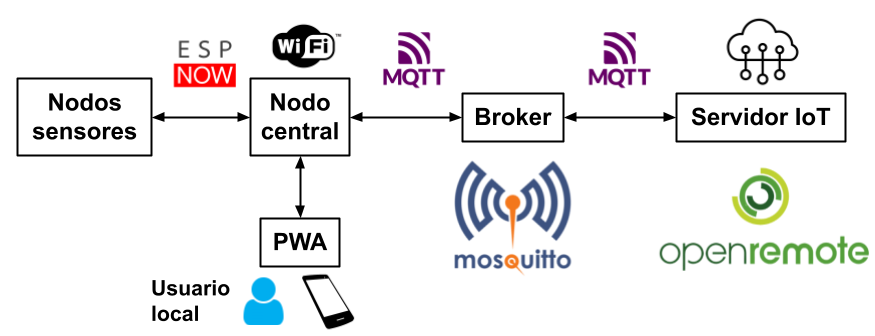
\includegraphics[width=1\textwidth]{./Figures/arq_sistema.png}
\caption{Esquema del sistema.}
\label{fig:arqSistema}
\end{figure}

En esta sección se describen los principales módulos que conforman el sistema, detallando su función y cómo interactúan entre sí.

\subsection{Nodos sensores} 

Están conformados por un módulo ESP32-C3 y un sensor. Esta es la capa de percepción, ya que los nodos son responsables de captar la información del entorno. Los datos recopilados son enviados al nodo central (gateway) a través del protocolo de comunicación ESP-NOW. En este contexto, también se incluye un módulo específico para gestionar los relés, cuyo estado puede ser consultado y modificado, por lo que se establece una \textit{comunicación bidireccional} con el \textit{gateway}. Sin embargo, en el caso de los sensores, la \textit{comunicación es unidireccional}, ya que solo envían datos.

\subsection{Nodo central}

Como se mencionó, este nodo se comunica con los sensores a través de ESP-NOW. Actúa como la capa de transporte, encargándose de transferir los datos capturados por la capa de percepción. Además, el \textit{gateway} integra una interfaz web embebida para visualizar los datos de los sensores y el estado de los relés. Esta interfaz está implementada utilizando un socket y, en caso de ausencia de conexión a internet, genera un “Access Point” (AP) local al cual el usuario puede conectarse para monitorear el estado del invernadero. El nodo central se conecta a internet mediante Wi-Fi para enviar los datos a un \textit{broker} MQTT (Mosquitto), empleando certificados TLS para asegurar la transmisión.

\subsection{Servidor IoT}

Este componente corresponde a la capa de procesamiento, donde se almacenan, analizan y gestionan los datos enviados desde el nodo central. Para esta función, se utilizará \textit{OpenRemote} como plataforma de servidor IoT, la cual facilita la integración de dispositivos y la gestión de datos. El servidor se conecta al \textit{broker} MQTT para recibir la información de los sensores y los relés.
Además de almacenar y visualizar los datos en tiempo real, el servidor permite generar informes, configurar alertas y ejecutar acciones automatizadas basadas en reglas predefinidas, como la activación de relés o notificaciones ante condiciones anómalas.



%----------------------------------------------------------------------------------------
\section{Desarrollo del firmware}

El \textit{firmware} del trabajo fue desarrollado utilizando el lenguaje de programación \textit{Python}, específicamente bajo el \textit{framework MicroPython}. Para su implementación, se empleó el entorno de desarrollo Visual Studio Code, que facilitó la edición y depuración del código.

En esta sección se presentan los diagramas de flujo que describen los procesos clave de los nodos sensores, el módulo de relés y el nodo central. Estos diagramas ilustran la lógica implementada en el \textit{firmware} y cómo se gestiona la comunicación eficiente entre sensores, actuadores, la interfaz web y el servidor IoT.

\subsection{Nodos sensores y módulo relés}

\subsubsection{Nodos sensores}

En la figura \ref{fig:flujoSensor} se presenta el diagrama de flujo de los nodos sensores. 

Cada sensor tendrá un script personalizado, ya que son diferentes entre sí, lo que implica que la forma de obtener las lecturas de los datos variará en cada caso. Sin embargo, el procedimiento para enviar los datos será el mismo para todos.

Primero, se inicializa y configura ESP-NOW para enviar mensajes en modo \textit{broadcast} (difusión) a todos los dispositivos cercanos, sin la necesidad de conocer sus direcciones MAC individuales
A continuación, el nodo busca el canal en el que se encuentra el \textit{gateway}. Una vez encontrado, se envía un mensaje de verificación para confirmar que el canal es el correcto. Si no se recibe respuesta, el nodo se reinicia, comenzando el proceso nuevamente.

Cuando el canal es verificado, se toma la lectura de los datos del sensor y se envía esta información al \textit{gateway} vía ESP-NOW, de forma encriptada, utilizando una librería específica de \textit{MicroPython} llamada \textit{cryptolib} \citep{docsmpy}.

Una vez que la información ha sido enviada, el dispositivo entra en \textit{modo DeepSleep} (sueño profundo) durante un tiempo determinado, con el fin de ahorrar energía. Al despertar, el módulo se reinicia como si hubiese sido encendido nuevamente.

\begin{figure}[H]
\centering 
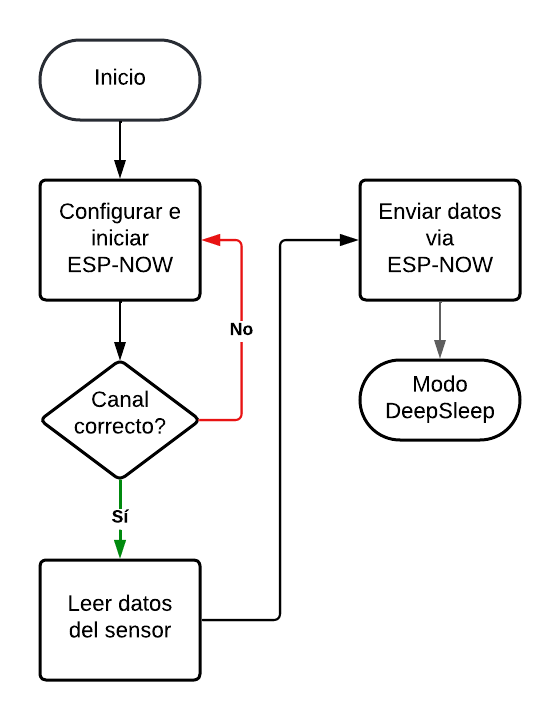
\includegraphics[width=0.5\textwidth]{./Figures/flujo_nodo_sensor.png}
\caption{Diagrama de flujo de los nodos sensores.}
\label{fig:flujoSensor}
\end{figure}

\subsubsection{Módulo relés}

El nodo encargado de los relés sigue un funcionamiento similar al de los nodos sensores en cuanto a la configuración inicial de ESP-NOW, por lo que no es necesario volver a detallar ese proceso. La principal diferencia radica en que, en lugar de tomar lecturas de un sensor, este nodo inicializa los relés y envía el estado en el que se encuentran al \textit{gateway}.

Una vez enviados los estados, el nodo queda a la espera de recibir instrucciones para modificar alguno de los relés. Si se recibe una solicitud para cambiar el estado de uno o más relés, el nodo ejecuta el cambio y, a continuación, envía nuevamente la información actualizada al \textit{gateway}.
Al igual que en los nodos sensores, la información se envía de forma encriptada para garantizar la seguridad de los datos transmitidos. De la misma manera, cualquier información que llega al nodo, como instrucciones para cambiar el estado de los relés, es desencriptada antes de ser procesada.

Este nodo no entra en \textit{modo DeepSleep}, ya que es necesario garantizar que los relés respondan de manera inmediata a cualquier instrucción de control que pueda recibirse.

En la figura \ref{fig:flujoRele} se puede observar el diagrama de flujo del módulo relés. 

\begin{figure}[H]
\centering 
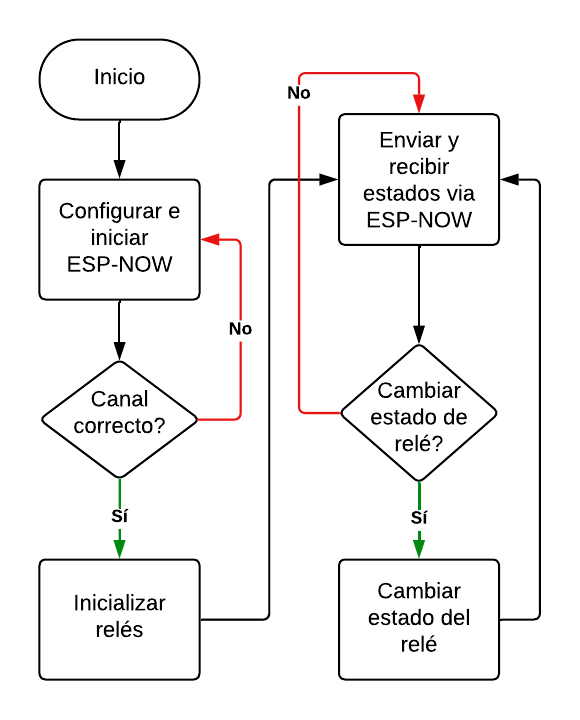
\includegraphics[width=0.5\textwidth]{./Figures/flujo_rele.png}
\caption{Diagrama de flujo del módulo relés.}
\label{fig:flujoRele}
\end{figure}

\subsection{Nodo Central}

El \textit{gateway} puede iniciar en dos modos diferentes: \textit{Modo Cliente} (CL) o \textit{Modo Access Point} (AP), dependiendo de la configuración cargada en el dispositivo. Una vez determinado el modo de operación, se configura e inicia la comunicación ESP-NOW en \textit{modo de difusión}.

\begin{itemize}
	\item Modo AP: en este caso, el \textit{gateway} actúa como un punto de acceso local, lo que significa que no está conectado a internet. Se inicia el servidor HTTP para proporcionar una interfaz web accesible a través de una red local, permitiendo al usuario monitorear y gestionar el sistema directamente sin necesidad de conexión externa.
	\item Modo CL: al iniciar en este modo significa que está conectado a internet a través de una red Wi-Fi. Se establece una conexión segura con un \textit{broker} MQTT. Para ello, se utilizan un nombre de usuario, una contraseña y certificados TLS para asegurar la comunicación. Además, el gateway se suscribe a un tópico específico del \textit{broker} MQTT, lo que le permite recibir mensajes relacionados con los sensores. Por último se inicia el servidor HTTP, lo que permite el acceso a la interfaz web embebida para monitorear y gestionar el sistema desde cualquier lugar con acceso a internet.
\end{itemize}

En la figura \ref{fig:flujoCentral} se puede observar el diagrama de flujo general del nodo central. 

\begin{figure}[H]
\centering 
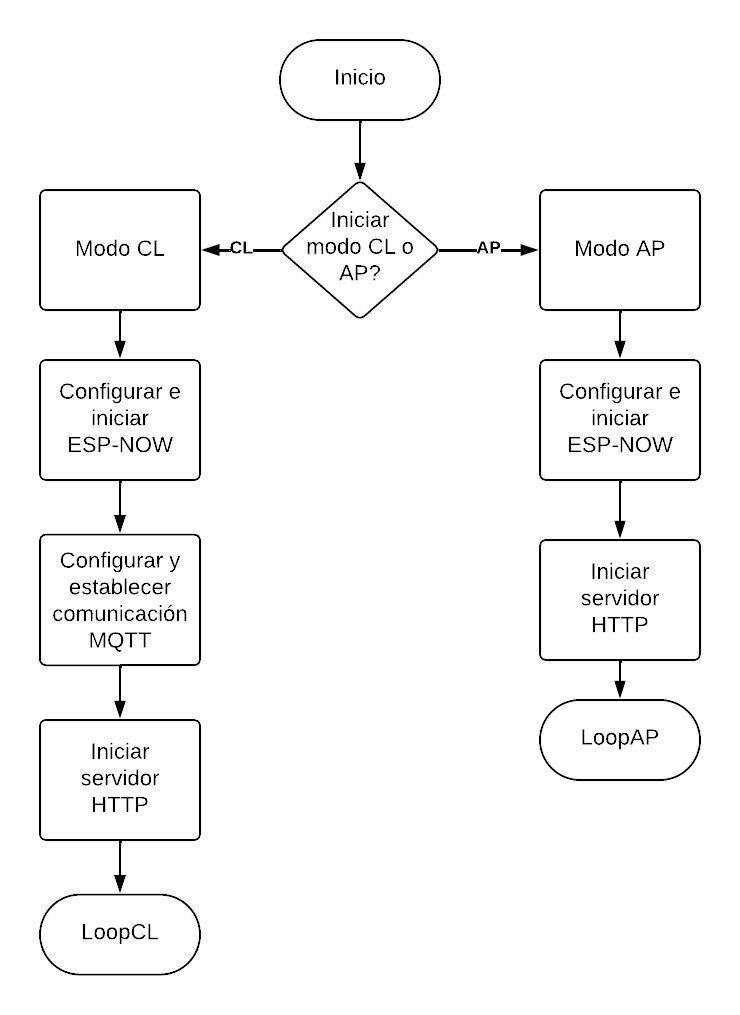
\includegraphics[width=0.7\textwidth]{./Figures/flujo_central.png}
\caption{Diagrama de flujo del nodo central.}
\label{fig:flujoCentral}
\end{figure}

\subsubsection{Loop AP}

En la figura \ref{fig:flujoAP} se puede observar el diagrama de flujo del loopAP. 

Una vez que el \textit{gateway} se ha iniciado en Modo AP y se ha configurado correctamente la comunicación ESP-NOW, entra en un bucle continuo de monitoreo y control, conocido como LoopAP. En este modo el \textit{gateway} realiza las siguientes acciones:

\begin{itemize}
	\item Monitoreo de nodos: el \textit{gateway} espera recibir datos de los nodos sensores y del módulo de relés a través de ESP-NOW. Al recibir información, ya sea de sensores o del estado de los relés, estos datos se envían y muestran en la PWA en tiempo real.
	\item Verificación de cambios en la PWA: si no se recibe información desde los nodos, el \textit{gateway} revisa si hubo un cambio en el estado de los relés en la PWA. Si detecta un cambio, envía la actualización al nodo correspondiente mediante ESP-NOW.
	\item Reinicio del ciclo: luego de procesar cualquier evento, el \textit{gateway} regresa al inicio del ciclo, quedando en espera de nuevos datos o cambios.
\end{itemize}


\begin{figure}[H]
\centering 
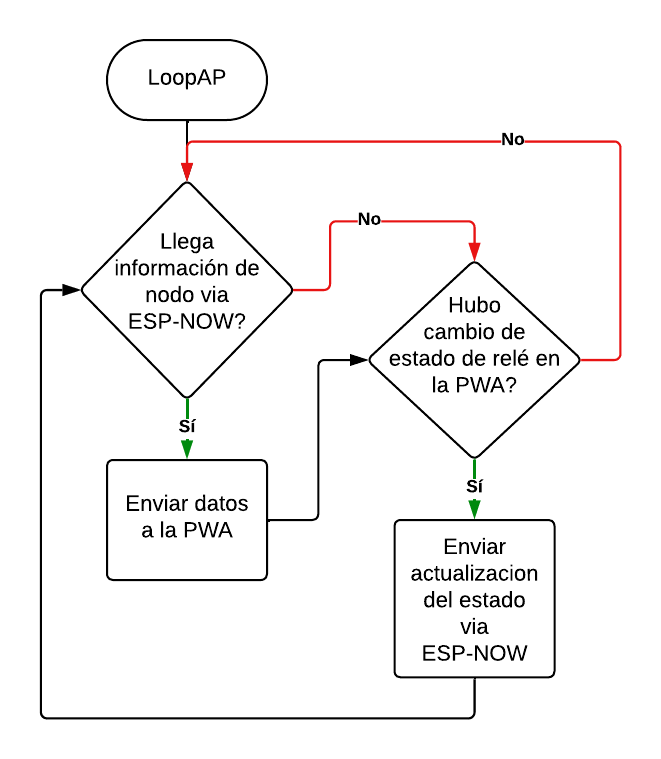
\includegraphics[width=0.5\textwidth]{./Figures/flujo_ap.png}
\caption{Diagrama de flujo del loop AP.}
\label{fig:flujoAP}
\end{figure}

\subsubsection{Loop CL}

En este modo, los datos de los sensores no solo se muestran localmente en la PWA, sino que también se publican en el \textit{broker} MQTT, lo que permite que sean almacenados y procesados remotamente. Esto garantiza una mayor capacidad de monitoreo y análisis.
Otra diferencia importante es la sincronización con el servidor IoT. Mientras que en el LoopAP los cambios en el estado de los relés solo se controlan desde la PWA, en el LoopCL también se monitorea si el estado de los relés ha sido modificado desde el servidor IoT. Esto posibilita la gestión remota de los dispositivos, permitiendo que el usuario controle y supervise el invernadero desde cualquier lugar con acceso a internet, una funcionalidad que no está disponible en el modo AP.

En la figura \ref{fig:flujoAP} se presenta el diagrama de flujo del loopCL. 

\begin{figure}[H]
\centering 
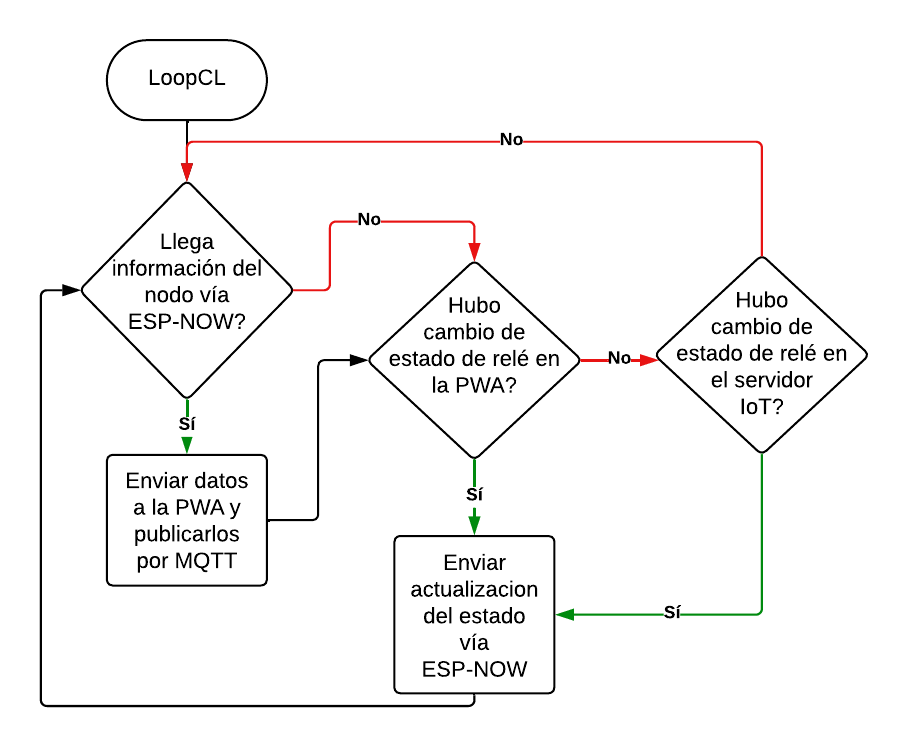
\includegraphics[width=0.6\textwidth]{./Figures/flujo_cl.png}
\caption{Diagrama de flujo del loop CL.}
\label{fig:flujoCL}
\end{figure}

%----------------------------------------------------------------------------------------
\section{Desarrollo de la aplicacion web progresiva}

%----------------------------------------------------------------------------------------
\section{Implementación del servidor IoT}

%----------------------------------------------------------------------------------------
\section{Despliegue del sistema}




% Chapter Template

\chapter{Ensayos y resultados} % Main chapter title

\label{Chapter4} % Change X to a consecutive number; for referencing this chapter elsewhere, use \ref{ChapterX}

%----------------------------------------------------------------------------------------
%	SECTION 1
%----------------------------------------------------------------------------------------

\section{Pruebas funcionales del hardware}
\label{sec:pruebasHW}

La idea de esta sección es explicar cómo se hicieron los ensayos, qué resultados se obtuvieron y analizarlos.
 
% Chapter Template

\chapter{Conclusiones} % Main chapter title

\label{Chapter5} % Change X to a consecutive number; for referencing this chapter elsewhere, use \ref{ChapterX}


%----------------------------------------------------------------------------------------

%----------------------------------------------------------------------------------------
%	SECTION 1
%----------------------------------------------------------------------------------------

\section{Conclusiones del trabajo realizado}

En la presente memoria de tesis se ha documentado el Trabajo Final para la obtención del grado de \degreename.  

Se obtuvo un \textit{firmware} que permite controlar un acuario en forma remota mediante una interfaz web embebida en la plataforma CIAA-NXP. Se aplicaron simplificaciones al modelo de acuario, principalmente debido a las restricciones de tiempo establecidas para la finalización del trabajo y a la ejecución de acciones de contingencia de riesgos identificados al comienzo de la planificación del trabajo, a saber:

\begin{itemize}
	\item Riesgo: No contar con un subsidio para la adquisición de sensores y actuadores de acuario.
	\item Riesgo: No disponer de una CIAA-NXP a tiempo para el comienzo del proyecto.
	\item Contingencia:  Simular sensores y actuadores del modelo de acuario.
\end{itemize}

Con las mencionadas simplificaciones se obtuvo una ``planta piloto'' que permitió avanzar en el desarrollo del \textit{firmware} de control y cumplir con los requerimientos de tiempo de finalización.

Se pudo integrar el \textit{stack} TCP/IP lwIP con el RTOS freeRTOS al \textit{firmware} de control sobre la base de un \textit{port} desarrollado por NXP, fabricante del microcontrolador LPC4337.

\medskip

Durante el desarrollo de este Trabajo Final se aplicaron conocimientos adquiridos a lo largo de la Carrera de Especialización en Sistemas Embebidos. Si bien el conjunto total de asignaturas cursadas aportaron conocimientos necesarios para la práctica profesional en el área de los Sistemas Embebidos, se quiere dejar constancia en particular, de las asignaturas con mayor relevancia para el trabajo presentado.

\begin{itemize}
\item
\textbf{Arquitectura de microprocesadores}. Resultó necesario tener conocimientos sobre la Arquitectura ARM Cortex M para la programación de la plataforma CIAA-NXP y el uso de los periféricos.

\item
\textbf{Programación de microprocesadores}. Se utilizaron buenas prácticas de programación de Lenguaje C para microcontroladores y periféricos, aprendidas en esta asignatura. Se empleó un formato de código consistente: comentarios en las declaraciones de funciones y partes importantes del código, constantes en mayúsculas, \textit{camelCase} para poner nombres significativos a funciones y variables. Se utilizaron APIs\footnote{\textit{Application Program Interface}} para abstraer distintas capas del código. Se obtuvo un código más legible y reutilizable.

\item
\textbf{Ingeniería de Software en Sistemas Embebidos}. Se utilizaron técnicas provenientes de la Ingeniería de Software. Siempre que fue posible se utilizó un método sistemático e iterativo de desarrollo pensando en el ciclo de vida del \textit{software}. Se hizo uso extensivo de Git como sistema de control de versiones del software.  Asimismo, se aplicaron metodologías de ensayo de \textit{software} aprendidas en esta asignatura.

\item
\textbf{Gestión de Proyectos en Ingeniería}. Resultó de gran utilidad elaborar un Plan de Proyecto para organizar el Trabajo Final.  Parte del material elaborado en esta asignatura como la planificación y el desglose de tareas se pueden encontrar en la presente memoria, en el capítulo \ref{Chapter2}.

\item
\textbf{Sistemas Operativos de Tiempo Real (I y II)}. Se aplicaron los conocimientos adquiridos sobre freeRTOS respecto a tareas, cambios de contexto y semáforos entre otros.  Asimismo, se utilizaron herramientas de desarrollo propias de freeRTOS para medir el uso de las pilas de las tareas creadas y optimizar el uso de la memoria.

\item 
\textbf{Protocolos de Comunicación}. Se aplicaron ampliamente los conocimientos obtenidos en el área de Ethernet. En particular, resultó útil el material sobre el \textit{stack} TCP/IP lwIP.

\item
\textbf{Diseño de Sistemas Críticos}. Siempre que fue posible se utilizaron técnicas de programación defensiva para que el comportamiento del \textit{firmware} resulte lo más predecible posible.  Se buscó obtener un sistema de control que no falle en primer lugar, y que si lo hace, falle en forma segura evitando daños tanto a los seres vivos dentro y fuera del acuario como a la propiedad.
\end{itemize}



\medskip

\noindent Asimismo, durante el desarrollo del trabajo final se adquirieron conocimientos en las áreas de:

\begin{itemize}
	\item Programación en lenguaje HTML5.
	\item Programación en lenguaje JavaScript.  
	\item Utilización de \textit{linker scripts} para el entorno de desarrollo LPCXpresso.
\end{itemize}


\medskip

Por lo tanto, se concluye que los objetivos planteados al comienzo del trabajo han sido alcanzados satisfactoriamente, habiéndose cumplido con los criterios de aceptación del sistema final y además, se han obtenido conocimientos valiosos para la formación profesional del autor.

%----------------------------------------------------------------------------------------
%	SECTION 2
%----------------------------------------------------------------------------------------
\clearpage
\section{Trabajo futuro}

Se considera oportuno identificar las líneas de trabajo futuro para dar continuidad al esfuerzo invertido.  Se listan a continuación las principales.

\begin{itemize}
	\item Trabajar con una planta piloto real, con sensores y actuadores de acuario.  Caracterizar la dinámica del entorno real y ajustar la lógica de control si fuera necesario.
	\vspace{5px}
	\item Escalar el \textit{firmware} desarrollado para obtener un \textit{framework} que posibilite cambiar el dominio de aplicación a otras áreas de control donde el modelo de ``medir, alertar y actuar'' aplique.
	\vspace{5px}
	\item Permitir la introducción de nuevos sensores y actuadores debidamente parametrizados mediante la interfaz de usuario.
	\vspace{5px}
	\item Mejorar la portabilidad de la interfaz web utilizando técnicas de RWD (\textit{Responsive Web Design}) para que permita su correcta visualización en distintos dispositivos, navegadores y resoluciones de pantalla.
\end{itemize}






 

%----------------------------------------------------------------------------------------
%	CONTENIDO DE LA MEMORIA  - APÉNDICES
%----------------------------------------------------------------------------------------

\appendix % indicativo para indicarle a LaTeX los siguientes "capítulos" son apéndices

% Incluir los apéndices de la memoria como archivos separadas desde la carpeta Appendices
% Descomentar las líneas a medida que se escriben los apéndices

%% Appendix A

\chapter{Appendix Title Here} % Main appendix title

\label{AppendixA} % For referencing this appendix elsewhere, use \ref{AppendixA}

Write your Appendix content here.
%\include{Appendices/AppendixB}
%\include{Appendices/AppendixC}

%----------------------------------------------------------------------------------------
%	BIBLIOGRAPHY
%----------------------------------------------------------------------------------------

\Urlmuskip=0mu plus 1mu\relax
\raggedright
\printbibliography[heading=bibintoc]

%----------------------------------------------------------------------------------------

\end{document}  
